% Week 9: Decoding Strategies (Enhanced 2025)
% BSc Discovery Two-Tier: 25 main + 19 appendix = 44 slides
% Journey context + Quality-diversity hook + Contrastive search + Task recommendations
% Enhanced: November 9, 2025

% Master Template for NLP Course
% Optimal Readability Layout Standard
% All presentations should include this template

\documentclass[8pt,aspectratio=169]{beamer}
\usetheme{Madrid}
\setbeamertemplate{navigation symbols}{}

% ====================================
% OPTIMAL READABILITY COLOR PALETTE
% ====================================
\definecolor{PureBlack}{HTML}{000000}      % Main text (21:1 contrast)
\definecolor{DeepBlue}{HTML}{003D7A}       % Primary accent (12.6:1 contrast)
\definecolor{DarkGray}{HTML}{4A4A4A}       % Secondary text (9.7:1 contrast)
\definecolor{LightGray}{HTML}{E5E5E5}      % Borders and grids
\definecolor{ChartBlue}{HTML}{0066CC}      % Chart primary
\definecolor{ChartOrange}{HTML}{FF8800}    % Chart secondary
\definecolor{ChartTeal}{HTML}{00A0A0}      % Chart tertiary
\definecolor{ChartPurple}{HTML}{8B4789}    % Chart quaternary
\definecolor{DarkGreen}{HTML}{228B22}      % Success/positive
\definecolor{DarkRed}{HTML}{CC0000}        % Warning/negative

% ====================================
% BEAMER COLOR CONFIGURATION
% ====================================
\setbeamercolor{structure}{fg=PureBlack}
\setbeamercolor{frametitle}{fg=PureBlack,bg=white}
\setbeamercolor{title}{fg=PureBlack,bg=white}
\setbeamercolor{subtitle}{fg=DarkGray}
\setbeamercolor{author}{fg=DarkGray}
\setbeamercolor{date}{fg=DarkGray}
\setbeamercolor{institute}{fg=DarkGray}

% Blocks - no backgrounds
\setbeamercolor{block title}{fg=PureBlack,bg=white}
\setbeamercolor{block body}{fg=PureBlack,bg=white}
\setbeamercolor{block title example}{fg=DarkGreen,bg=white}
\setbeamercolor{block body example}{fg=PureBlack,bg=white}
\setbeamercolor{block title alerted}{fg=DarkRed,bg=white}
\setbeamercolor{block body alerted}{fg=PureBlack,bg=white}

% Lists
\setbeamercolor{item}{fg=DeepBlue}
\setbeamercolor{subitem}{fg=ChartBlue}
\setbeamercolor{enumerate item}{fg=DeepBlue}
\setbeamercolor{enumerate subitem}{fg=ChartBlue}

% Text
\setbeamercolor{normal text}{fg=PureBlack,bg=white}
\setbeamercolor{alerted text}{fg=DarkRed}
\setbeamercolor{example text}{fg=DarkGreen}

% Footer
\setbeamercolor{footline}{fg=DarkGray,bg=white}
\setbeamercolor{page number in head/foot}{fg=DarkGray}

% ====================================
% FONT CONFIGURATION
% ====================================
\setbeamerfont{normal text}{size=\normalsize}
\setbeamerfont{frametitle}{size=\Large,series=\bfseries}
\setbeamerfont{title}{size=\huge,series=\bfseries}
\setbeamerfont{subtitle}{size=\large}
\setbeamerfont{author}{size=\normalsize}
\setbeamerfont{date}{size=\small}
\setbeamerfont{institute}{size=\small}

% ====================================
% REQUIRED PACKAGES
% ====================================
\usepackage{tikz}
\usepackage{amsmath}
\usepackage{amssymb}
\usepackage{booktabs}
\usepackage{graphicx}
\usepackage{array}
\usepackage{listings}
\usepackage{algorithm2e}
\usepackage{xcolor}
\usepackage{tabularx}
\usepackage{multirow}
\usepackage{subcaption}

% ====================================
% CUSTOM COMMANDS
% ====================================
% Text highlighting commands
\newcommand{\highlight}[1]{\textcolor{DeepBlue}{\textbf{#1}}}
\newcommand{\secondary}[1]{\textcolor{DarkGray}{#1}}
\newcommand{\success}[1]{\textcolor{DarkGreen}{#1}}
\newcommand{\warning}[1]{\textcolor{DarkRed}{#1}}
\newcommand{\data}[1]{\textcolor{ChartBlue}{#1}}
\newcommand{\dataalt}[1]{\textcolor{ChartOrange}{#1}}

% Mathematical notation
\newcommand{\given}{\mid}
\newcommand{\prob}[1]{P(#1)}
\newcommand{\argmax}{\operatorname*{argmax}}
\newcommand{\argmin}{\operatorname*{argmin}}
\newcommand{\softmax}{\operatorname{softmax}}

% Box commands for emphasis
\newcommand{\keypoint}[1]{%
  \begin{center}
  \fbox{\parbox{0.9\textwidth}{\centering\textbf{#1}}}
  \end{center}
}

\newcommand{\formula}[1]{%
  \begin{center}
  \colorbox{LightGray}{\parbox{0.8\textwidth}{\centering$\displaystyle #1$}}
  \end{center}
}

% ====================================
% LISTINGS CONFIGURATION
% ====================================
\lstset{
  basicstyle=\ttfamily\small,
  keywordstyle=\color{DeepBlue}\bfseries,
  commentstyle=\color{DarkGray}\itshape,
  stringstyle=\color{ChartOrange},
  numbers=left,
  numberstyle=\tiny\color{DarkGray},
  stepnumber=1,
  numbersep=5pt,
  backgroundcolor=\color{white},
  showspaces=false,
  showstringspaces=false,
  showtabs=false,
  frame=single,
  frameround=tttt,
  rulecolor=\color{LightGray},
  tabsize=2,
  captionpos=b,
  breaklines=true,
  breakatwhitespace=true,
  language=Python,
  escapeinside={(*@}{@*)},
  morekeywords={self, yield, assert, with, as}
}

% ====================================
% STANDARD SLIDE LAYOUTS
% ====================================

% Two-column layout with title
\newcommand{\twocolslide}[3]{%
  \begin{frame}{#1}
  \begin{columns}[T]
  \column{0.48\textwidth}
  #2
  \column{0.48\textwidth}
  #3
  \end{columns}
  \end{frame}
}

% Three-column layout
\newcommand{\threecolslide}[4]{%
  \begin{frame}{#1}
  \begin{columns}[T]
  \column{0.32\textwidth}
  #2
  \column{0.32\textwidth}
  #3
  \column{0.32\textwidth}
  #4
  \end{columns}
  \end{frame}
}

% Chart slide with caption
\newcommand{\chartslide}[3]{%
  \begin{frame}{#1}
  \begin{center}
  \includegraphics[width=#2\textwidth]{#3}
  \end{center}
  \end{frame}
}

% Full chart slide - optimized to 0.85 for proper margins
\newcommand{\fullchartslide}[2]{%
  \begin{frame}{#1}
  \begin{center}
  \includegraphics[width=0.85\textwidth]{#2}
  \end{center}
  \end{frame}
}

% Code slide
\newcommand{\codeslide}[3]{%
  \begin{frame}[fragile]{#1}
  \begin{lstlisting}[language=#2]
#3
  \end{lstlisting}
  \end{frame}
}

% Concept slide with figure
\newcommand{\conceptslide}[3]{%
  \begin{frame}{#1}
  \begin{columns}[T]
  \column{0.6\textwidth}
  #2
  \column{0.35\textwidth}
  \begin{center}
  \includegraphics[width=0.95\textwidth]{#3}
  \end{center}
  \end{columns}
  \end{frame}
}

% Table slide
\newcommand{\tableslide}[2]{%
  \begin{frame}{#1}
  \begin{center}
  \Large
  \renewcommand{\arraystretch}{1.5}
  #2
  \end{center}
  \end{frame}
}

% Summary slide
\newcommand{\summaryslide}[2]{%
  \begin{frame}{#1}
  \begin{center}
  \Large
  #2
  \end{center}
  \vfill
  \begin{center}
  \keypoint{Key Takeaway}
  \end{center}
  \end{frame}
}

% ====================================
% REMOVE DECORATIONS
% ====================================
\setbeamertemplate{blocks}[default]
\setbeamertemplate{title page}[default][colsep=-4bp,rounded=false]
\setbeamertemplate{itemize items}[circle]
\setbeamertemplate{enumerate items}[default]
\setbeamertemplate{section in toc}[sections numbered]
\setbeamertemplate{subsection in toc}[subsections numbered]

% ====================================
% PAGE NUMBERING
% ====================================
\setbeamertemplate{footline}{
  \leavevmode%
  \hbox{%
  \begin{beamercolorbox}[wd=.333333\paperwidth,ht=2.25ex,dp=1ex,center]{author in head/foot}%
    \usebeamerfont{author in head/foot}\secondary{\insertshortauthor}
  \end{beamercolorbox}%
  \begin{beamercolorbox}[wd=.333333\paperwidth,ht=2.25ex,dp=1ex,center]{title in head/foot}%
    \usebeamerfont{title in head/foot}\secondary{\insertshorttitle}
  \end{beamercolorbox}%
  \begin{beamercolorbox}[wd=.333333\paperwidth,ht=2.25ex,dp=1ex,right]{date in head/foot}%
    \usebeamerfont{date in head/foot}\secondary{\insertshortdate{}\hspace*{2em}
    \insertframenumber{} / \inserttotalframenumber\hspace*{2ex}}
  \end{beamercolorbox}}%
  \vskip0pt%
}

% ====================================
% TABLE OF CONTENTS STYLE
% ====================================
\setbeamertemplate{section in toc}{%
  \leavevmode\leftskip=1.5em%
  \llap{%
    \usebeamerfont{section in toc}%
    \usebeamercolor[fg]{section in toc}%
    \inserttocsectionnumber.%
  }%
  \usebeamerfont{section in toc}%
  \usebeamercolor[fg]{section in toc}%
  \inserttocsection\par%
}

\setbeamertemplate{subsection in toc}{%
  \leavevmode\leftskip=3em%
  \llap{%
    \usebeamerfont{subsection in toc}%
    \usebeamercolor[fg]{subsection in toc}%
    \inserttocsectionnumber.\inserttocsubsectionnumber%
  }%
  \usebeamerfont{subsection in toc}%
  \usebeamercolor[fg]{subsection in toc}%
  \inserttocsubsection\par%
}

% ====================================
% END OF MASTER TEMPLATE
% ====================================

% Template beamer final styling
\definecolor{mllavender}{RGB}{173,173,224}
\definecolor{mllavender2}{RGB}{193,193,232}
\definecolor{mllavender3}{RGB}{204,204,235}

\newcommand{\bottomnote}[1]{%
\vfill
\vspace{-2mm}
\textcolor{mllavender2}{\rule{\textwidth}{0.4pt}}
\vspace{1mm}
\footnotesize
\textbf{#1}
}

\title{Decoding Strategies}
\subtitle{\secondary{Week 9 - From Prediction to Generation}}
\author{NLP Course 2025}
\date{November 9, 2025}

\begin{document}

% ============================================
% MAIN PRESENTATION (25 SLIDES)
% ============================================

\begin{frame}
\titlepage
\vfill
\begin{center}\secondary{\footnotesize Two-Tier BSc Discovery | Enhanced with Contrastive Search (2025)}\end{center}
\end{frame}

% === CONTEXT: HOW WE GOT HERE (2 NEW SLIDES) ===

\begin{frame}[t]{How We Got Here: The Prediction Story}
\vspace{-0.3cm}
\begin{center}
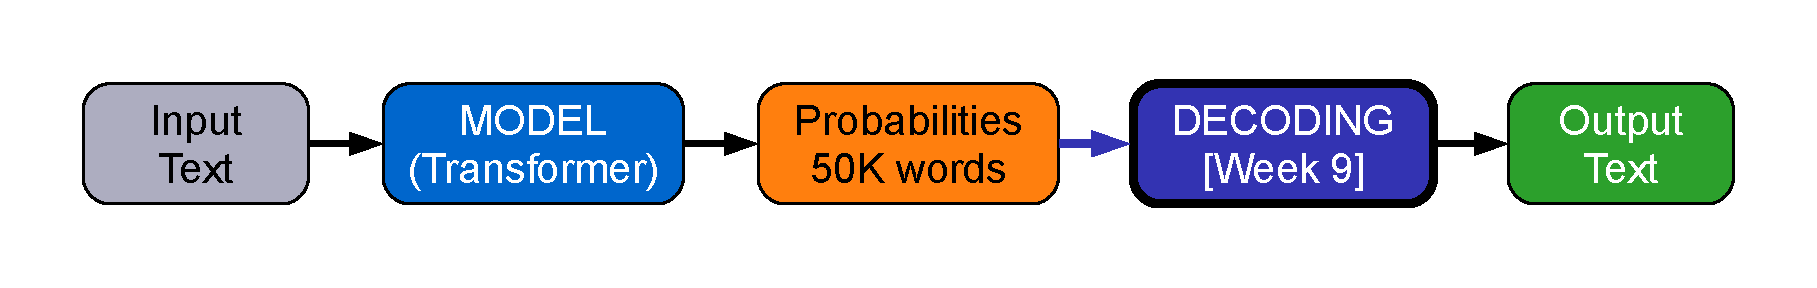
\includegraphics[width=0.75\textwidth]{../figures/prediction_to_text_pipeline_bsc.pdf}
\end{center}

\vspace{3mm}
\small
\textbf{Our Journey}:
\begin{enumerate}
\item We trained models (Weeks 3-7: RNN $\rightarrow$ Transformers $\rightarrow$ BERT/GPT)
\item They learned to predict: $P(\text{word} | \text{context})$
\item They output probability distributions over 50,000+ words
\item \textbf{Today}: How do we convert these probabilities into actual text?
\end{enumerate}

\bottomnote{Models predict probabilities. Decoding converts probabilities to text.}
\end{frame}

\begin{frame}[t]{Today's Challenge: From Probabilities to Text}
\small
\textbf{The Setup}: Model gives us probabilities for next word

\vspace{3mm}
Example: ``The cat \_\_''

$$P(\text{sat}) = 0.45, \quad P(\text{is}) = 0.30, \quad P(\text{jumped}) = 0.25, \quad ... \quad \text{(50,000 words)}$$

\vspace{5mm}
\begin{columns}[T]
\column{0.48\textwidth}
\textbf{Naive Approach 1}: Pick highest

$\rightarrow$ \textbf{Greedy Decoding}

\vspace{3mm}
\textbf{Result}:

``The city is a major city in the city...''

\vspace{3mm}
{\color{red}\textbf{Problem}}: Repetitive, boring, loops

\column{0.48\textwidth}
\textbf{Naive Approach 2}: Pick random

$\rightarrow$ \textbf{Pure Sampling}

\vspace{3mm}
\textbf{Result}:

``The purple flying mathematics yesterday...''

\vspace{3mm}
{\color{red}\textbf{Problem}}: Nonsense, incoherent
\end{columns}

\vspace{5mm}
\textbf{Core Challenge}: Need text that is \textit{coherent} AND \textit{creative}

\bottomnote{Today: 6 strategies to solve this challenge - from simple to sophisticated}
\end{frame}

% === HOOK (2 slides) ===

\begin{frame}[t]{The Quality-Diversity Tradeoff}
\vspace{-0.3cm}
\begin{center}
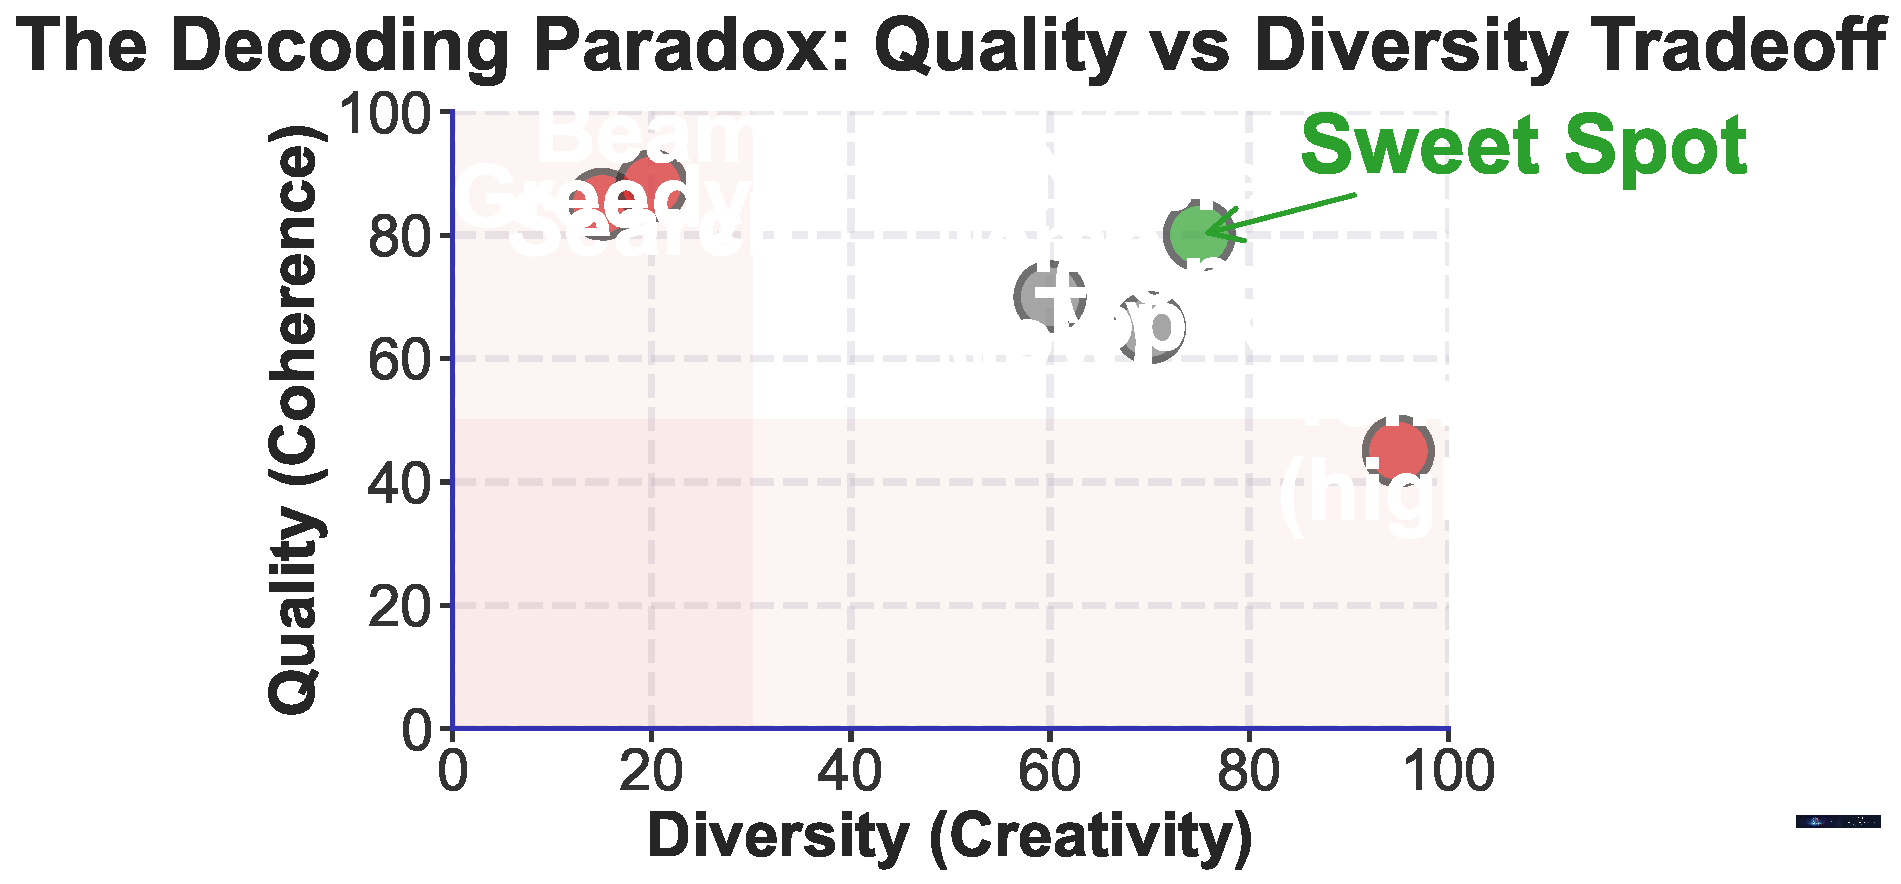
\includegraphics[width=0.70\textwidth]{../figures/quality_diversity_tradeoff_bsc.pdf}
\end{center}
\begin{center}
\textbf{Discovery Question}: Why is best text boring and creative text nonsense?
\end{center}
\bottomnote{The central challenge: How to balance coherence with creativity}
\end{frame}

\begin{frame}[t]{Three Decoding Families}
\small
\begin{columns}[T]
\column{0.32\textwidth}
\textbf{Deterministic}

\textbf{Methods}:
\begin{itemize}
\item Greedy
\item Beam search
\end{itemize}

\textbf{Traits}:
\begin{itemize}
\item Same output always
\item High quality
\item No creativity
\end{itemize}

\column{0.32\textwidth}
\textbf{Stochastic}

\textbf{Methods}:
\begin{itemize}
\item Temperature
\item Top-k
\item Nucleus (top-p)
\end{itemize}

\textbf{Traits}:
\begin{itemize}
\item Random sampling
\item Creative
\item Can be chaotic
\end{itemize}

\column{0.32\textwidth}
\textbf{Balanced}

\textbf{Methods}:
\begin{itemize}
\item Contrastive
\item Hybrid
\end{itemize}

\textbf{Traits}:
\begin{itemize}
\item Best of both
\item Avoid repetition
\item Modern standard
\end{itemize}
\end{columns}
\bottomnote{Different tasks need different strategies - no single best method}
\end{frame}

% === DETERMINISTIC METHODS (4 slides: 4-7) ===

\begin{frame}[t]{Greedy Decoding: The Baseline}
\small
\begin{columns}[T]
\column{0.49\textwidth}
\textbf{How It Works}:

\begin{enumerate}
\item Compute probabilities for next token
\item Pick token with highest probability
\item Add to sequence
\item Repeat until done
\end{enumerate}

\vspace{3mm}
\textbf{Example}:

$P(\text{cat}) = 0.45$ ← Pick this!

$P(\text{dog}) = 0.30$

$P(\text{bird}) = 0.25$

\column{0.49\textwidth}
\textbf{When to Use}:
\begin{itemize}
\item Code generation (correctness critical)
\item Short responses
\item Speed is critical
\item Need reproducibility
\end{itemize}

\vspace{3mm}
\textbf{Problem}:

Always picks same word → repetitive text

``The city is a city in a city...''

\vspace{3mm}
{\color{red}\textbf{Degeneration}}: Model gets stuck in loops

\end{columns}
\bottomnote{Simplest method but prone to repetition - need better strategies}
\end{frame}

\begin{frame}[t]{Beam Search: Explore Multiple Paths}
\vspace{-0.3cm}
\begin{center}
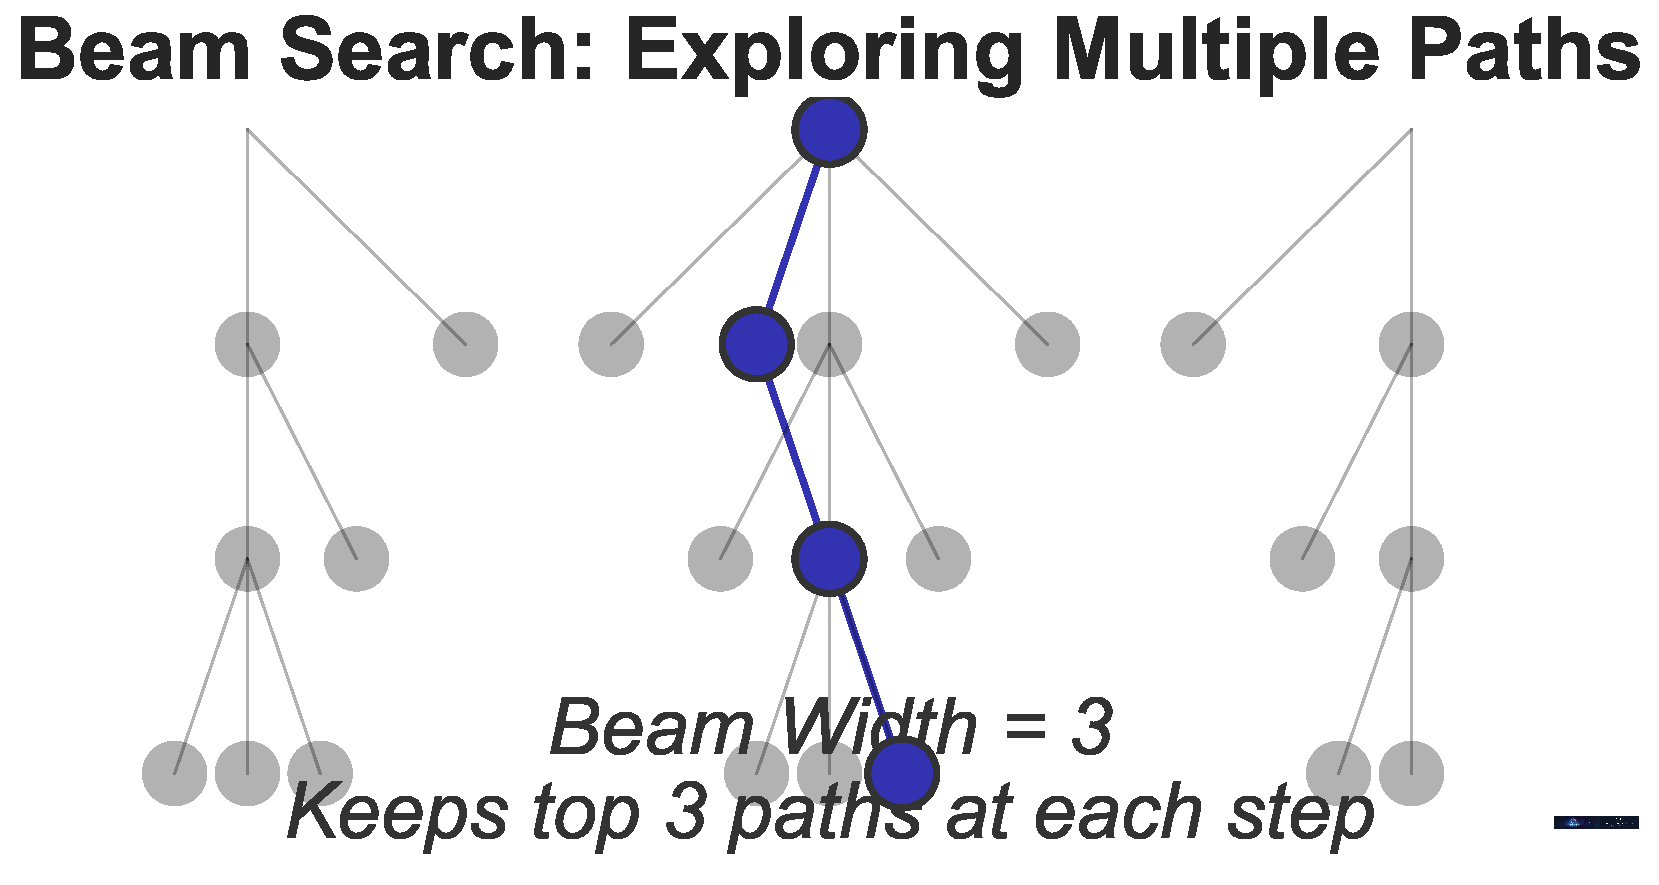
\includegraphics[width=0.70\textwidth]{../figures/beam_search_visual_bsc.pdf}
\end{center}
\begin{center}
\textbf{Key Insight}: Keep top-k hypotheses at each step to find better sequences
\end{center}
\bottomnote{Beam width = 3-5 typical. Balance between greedy (1) and exhaustive (all)}
\end{frame}

\begin{frame}[t]{Beam Search: Step-by-Step Example}
\vspace{-0.3cm}
\begin{center}
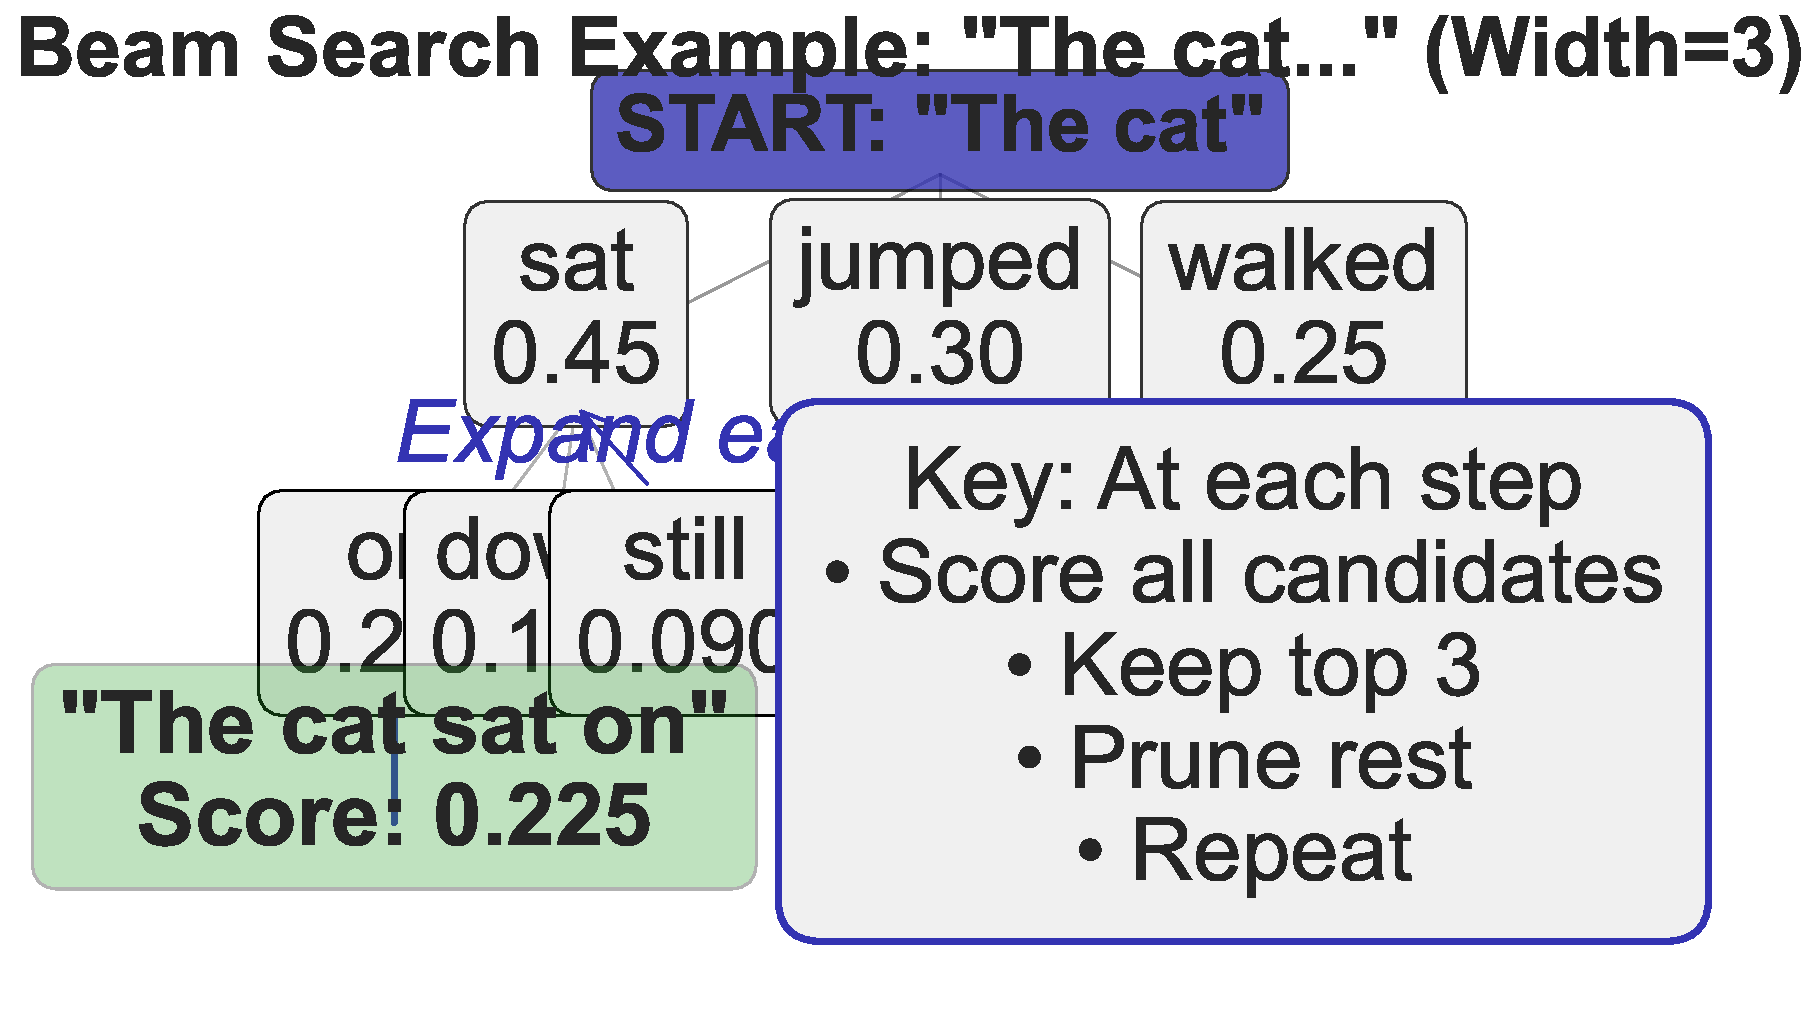
\includegraphics[width=0.75\textwidth]{../figures/beam_example_tree_bsc.pdf}
\end{center}
\bottomnote{Worked example shows why beam search finds better sequences than greedy}
\end{frame}

\begin{frame}[t]{Beam Search: Detail}
\small
\begin{columns}[T]
\column{0.49\textwidth}
\textbf{Algorithm}:

\begin{enumerate}
\item Start: Keep top-k tokens
\item Expand: Generate continuations for each
\item Score: Multiply probabilities
\item Prune: Keep top-k sequences
\item Repeat until END token
\end{enumerate}

\vspace{3mm}
\textbf{Scoring}:

$$\text{score}(y_1...y_t) = \prod_{i=1}^t P(y_i | y_{<i})$$

With length normalization:

$$\text{score} = \frac{1}{t} \sum_{i=1}^t \log P(y_i | y_{<i})$$

\column{0.49\textwidth}
\textbf{Best For}:
\begin{itemize}
\item Machine translation
\item Summarization
\item Question answering
\item Tasks with ``correct'' answer
\end{itemize}

\vspace{3mm}
\textbf{Parameters}:

Width = 3-5 (translation)

Width = 10 (diverse outputs)

\vspace{3mm}
\textbf{Tradeoffs}:

+ Better quality than greedy

+ Diverse hypotheses

- Still deterministic

- 4-5x slower than greedy

\end{columns}
\bottomnote{Beam search is the workhorse for deterministic tasks}
\end{frame}

% === STOCHASTIC METHODS (8 slides: 8-15) ===

\begin{frame}[t]{Temperature Sampling: Control Randomness}
\vspace{-0.3cm}
\begin{center}
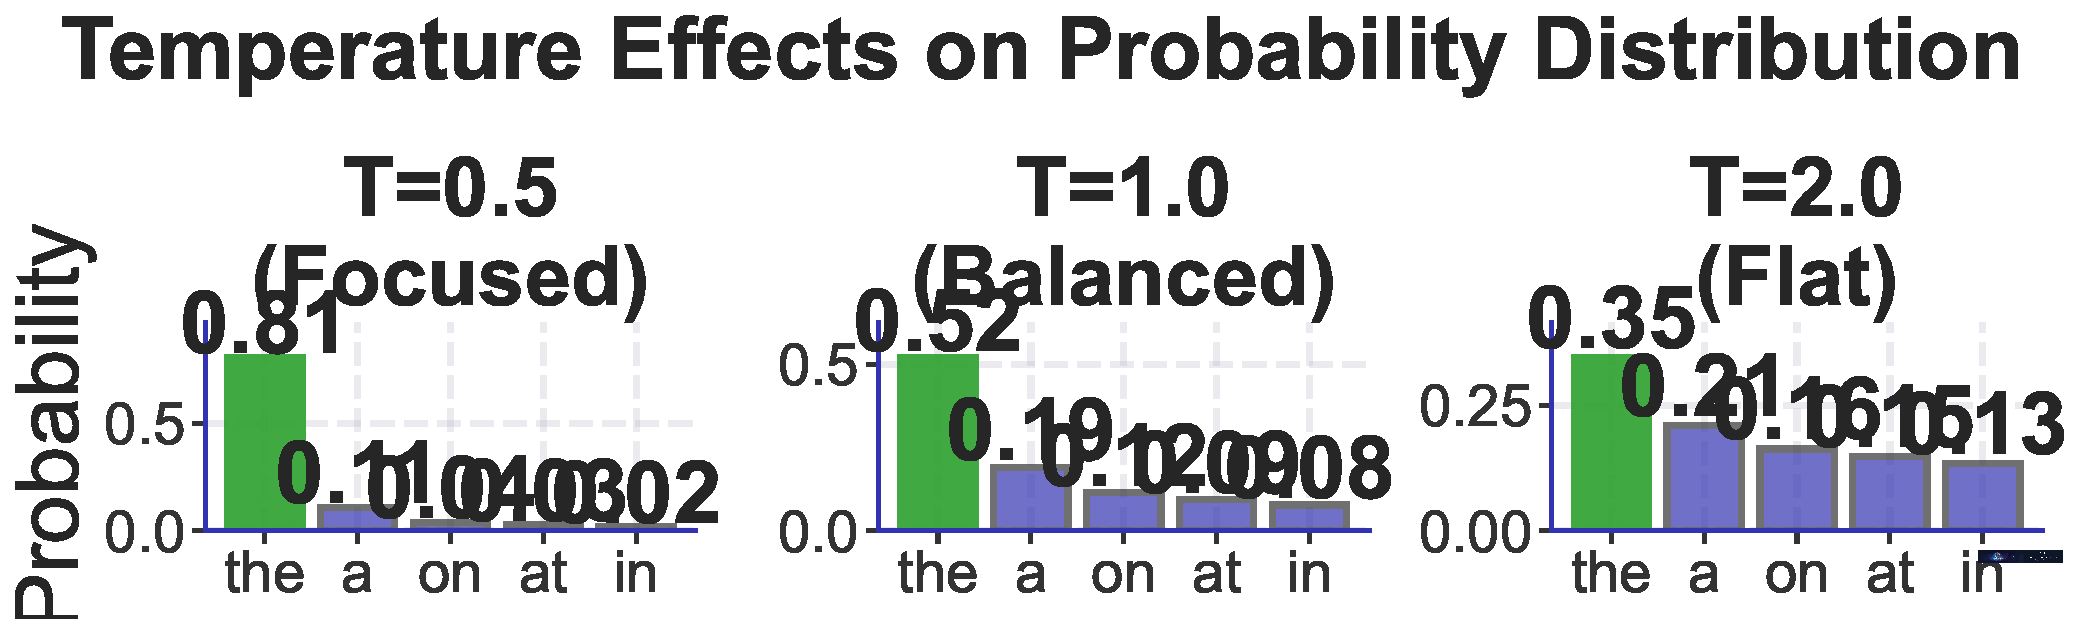
\includegraphics[width=0.65\textwidth]{../figures/temperature_effects_bsc.pdf}
\end{center}
\begin{center}
\textbf{Key Insight}: Temperature reshapes probability distribution
\end{center}
\bottomnote{T $<$ 1: more focused. T = 1: unchanged. T $>$ 1: more random}
\end{frame}

\begin{frame}[t]{Temperature: Worked Example}
\vspace{-0.3cm}
\begin{center}
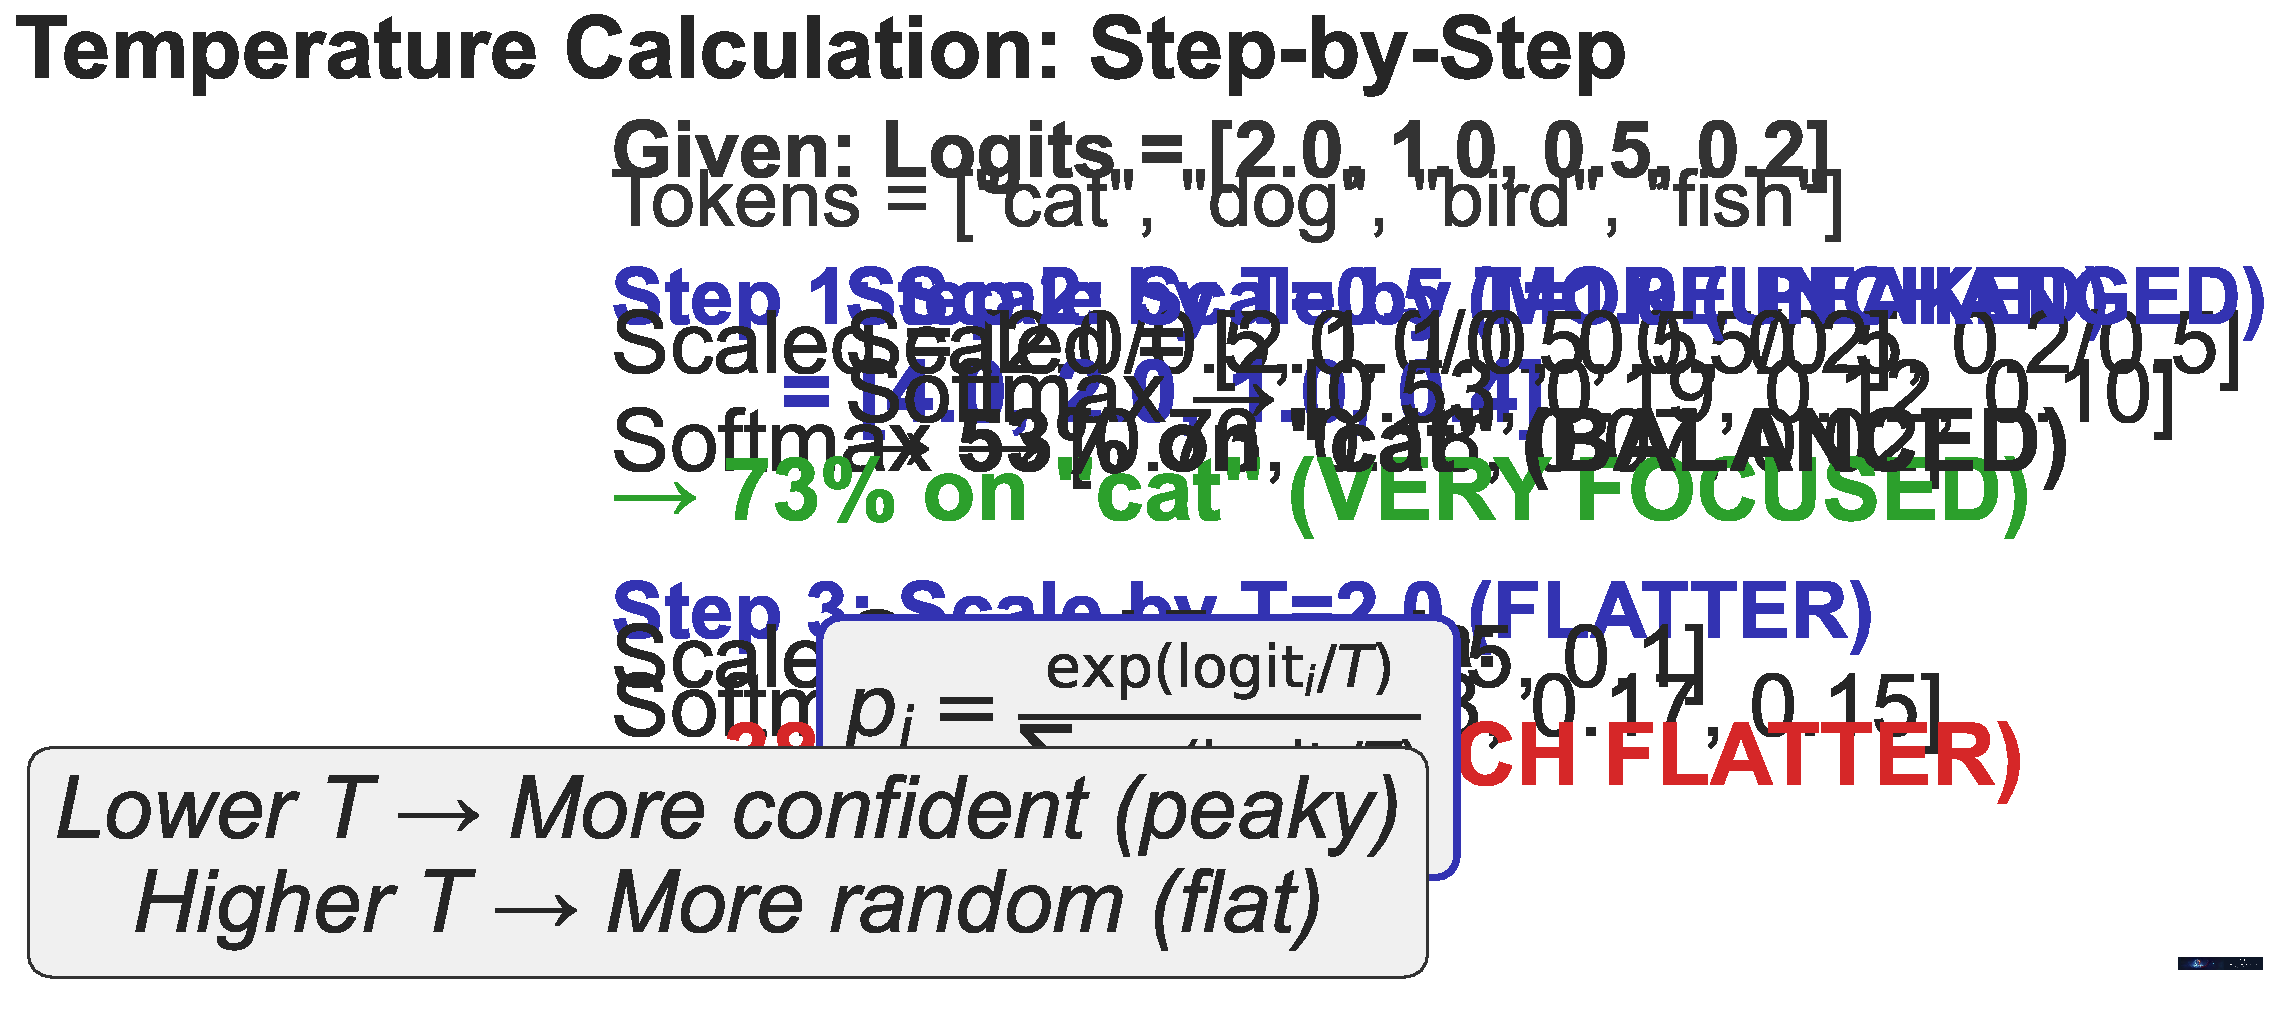
\includegraphics[width=0.70\textwidth]{../figures/temperature_calculation_bsc.pdf}
\end{center}
\bottomnote{Concrete numbers show how temperature scaling works}
\end{frame}

\begin{frame}[t]{Temperature: Detail}
\small
\begin{columns}[T]
\column{0.49\textwidth}
\textbf{How It Works}:

Given logits $z_1, z_2, ..., z_V$

\vspace{3mm}
Scale by temperature $T$:

$$p_i = \frac{\exp(z_i / T)}{\sum_j \exp(z_j / T)}$$

\vspace{3mm}
Sample from $p$

\vspace{3mm}
\textbf{Effect}:

$T \rightarrow 0$: argmax (greedy)

$T = 1$: standard softmax

$T \rightarrow \infty$: uniform

\column{0.49\textwidth}
\textbf{Practical Settings}:

\begin{itemize}
\item \textbf{T = 0.1-0.3}: Factual Q\&A
\item \textbf{T = 0.7}: Chatbots
\item \textbf{T = 0.9-1.2}: Creative writing
\item \textbf{T = 1.5+}: Experimental
\end{itemize}

\vspace{3mm}
\textbf{Tradeoffs}:

+ Simple to implement

+ Continuous control

- No quality guarantee

- Can generate nonsense

\end{columns}
\bottomnote{Temperature is the simplest randomness control}
\end{frame}

\begin{frame}[t]{Top-k Sampling: Filter the Tail}
\vspace{-0.3cm}
\begin{center}
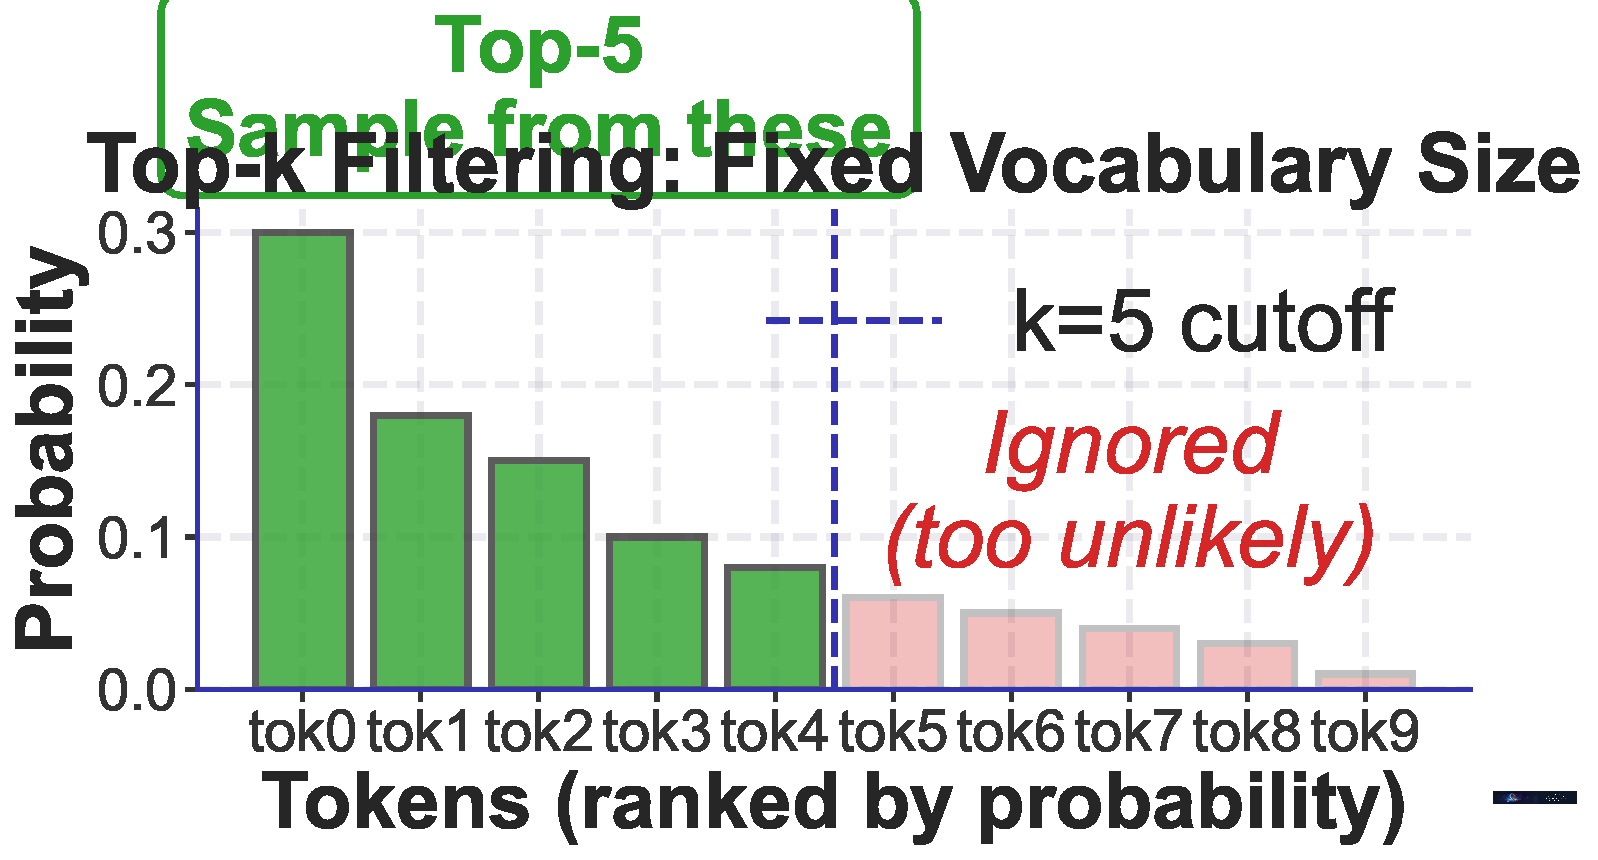
\includegraphics[width=0.70\textwidth]{../figures/topk_filtering_bsc.pdf}
\end{center}
\begin{center}
\textbf{Key Insight}: Only sample from top-k most likely tokens
\end{center}
\bottomnote{Prevents sampling from long tail of unlikely words}
\end{frame}

\begin{frame}[t]{Top-k: Worked Example (k=3)}
\vspace{-0.3cm}
\begin{center}
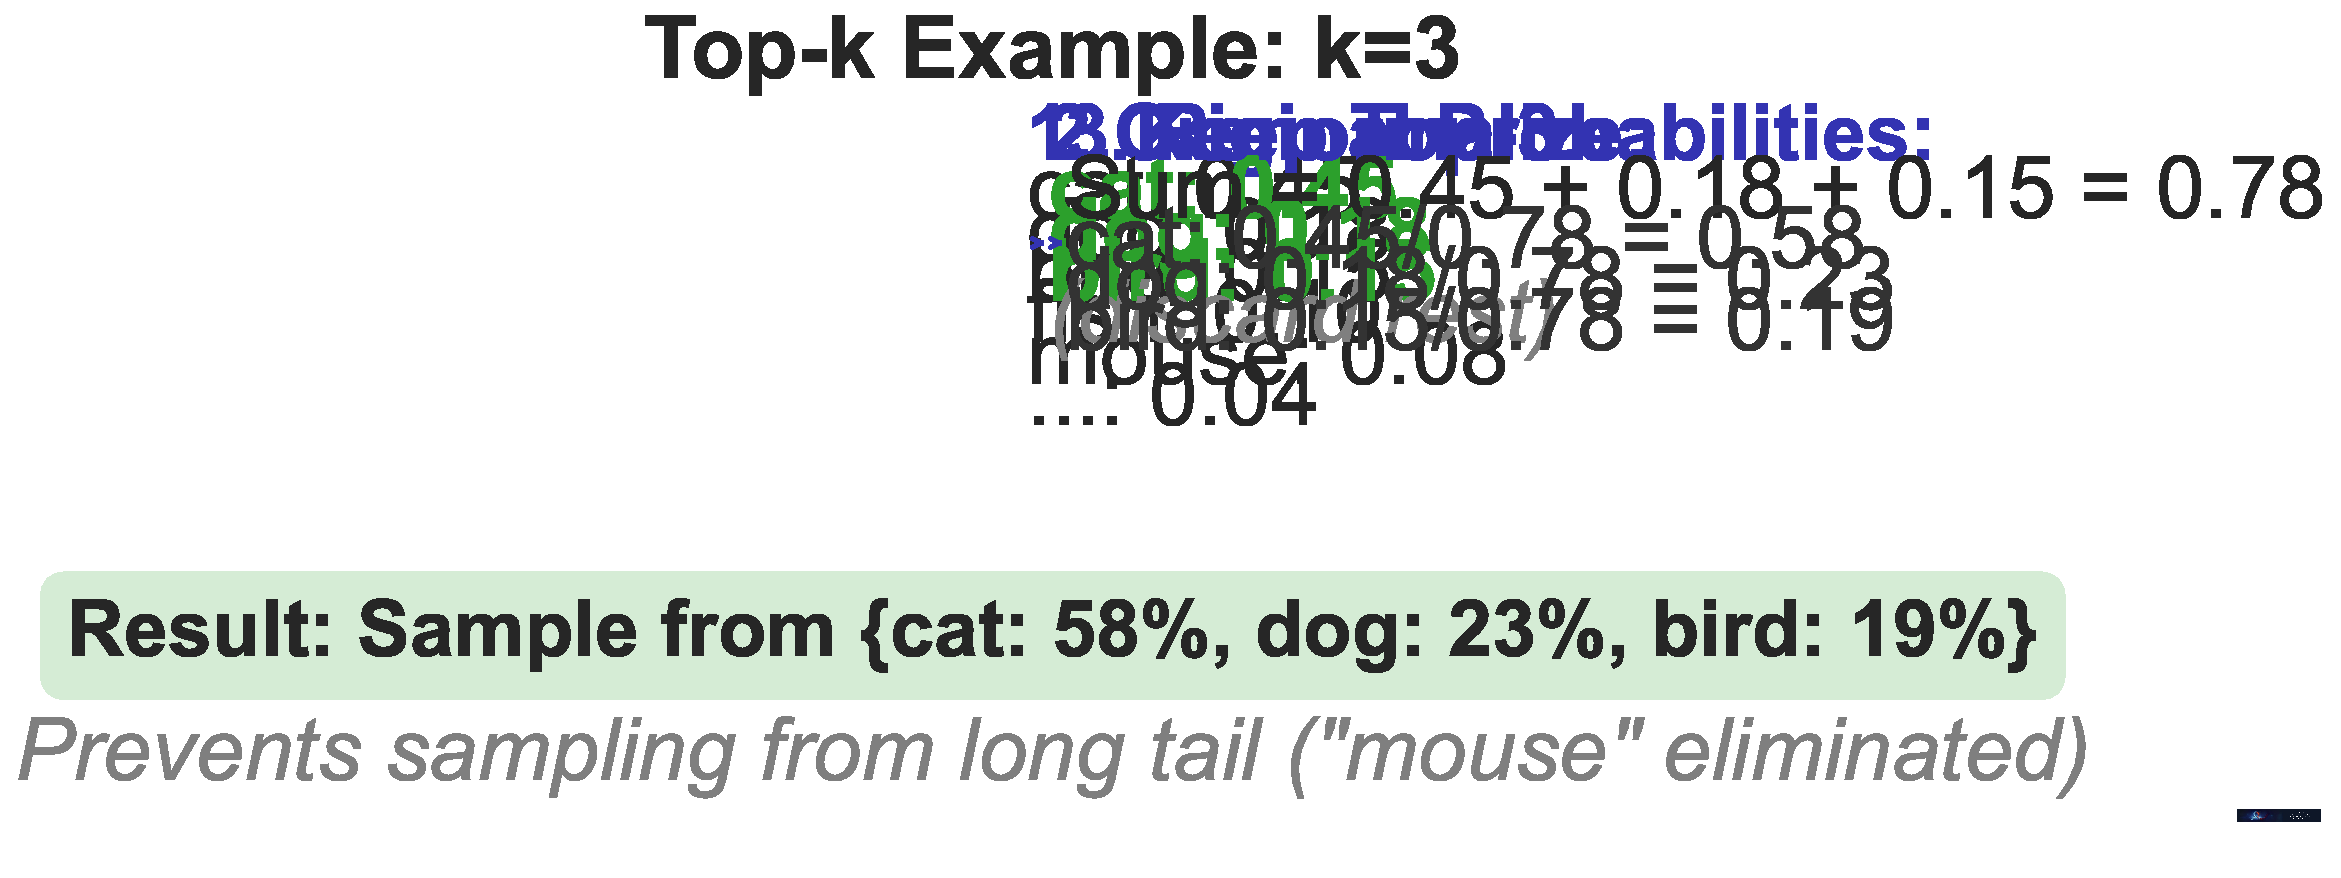
\includegraphics[width=0.70\textwidth]{../figures/topk_example_bsc.pdf}
\end{center}
\bottomnote{Filtering + renormalization prevents tail sampling}
\end{frame}

\begin{frame}[t]{Top-k: Detail}
\small
\begin{columns}[T]
\column{0.49\textwidth}
\textbf{Algorithm}:

\begin{enumerate}
\item Compute $P(w_i)$ for all tokens
\item Sort by probability
\item Keep only top-k
\item Renormalize: $p'_i = p_i / \sum_{j=1}^k p_j$
\item Sample from $p'$
\end{enumerate}

\vspace{3mm}
\textbf{Example} (k=3):

Original: [0.45, 0.18, 0.15, 0.10, ...]

Keep: [0.45, 0.18, 0.15]

Renormalize: [0.58, 0.23, 0.19]

\column{0.49\textwidth}
\textbf{Typical Values}:

k = 40-50 (balanced)

k = 10-20 (focused)

k = 100+ (very diverse)

\vspace{3mm}
\textbf{Limitation}:

Fixed cutoff regardless of distribution!

Peaked: Wastes probability mass

Flat: Still allows too many bad tokens

\vspace{3mm}
\textbf{Solution}: Dynamic cutoff (nucleus)

\end{columns}
\bottomnote{Top-k improves over temperature but fixed cutoff is inflexible}
\end{frame}

\begin{frame}[t]{Nucleus (Top-p) Sampling: Dynamic Cutoff}
\vspace{-0.3cm}
\begin{center}
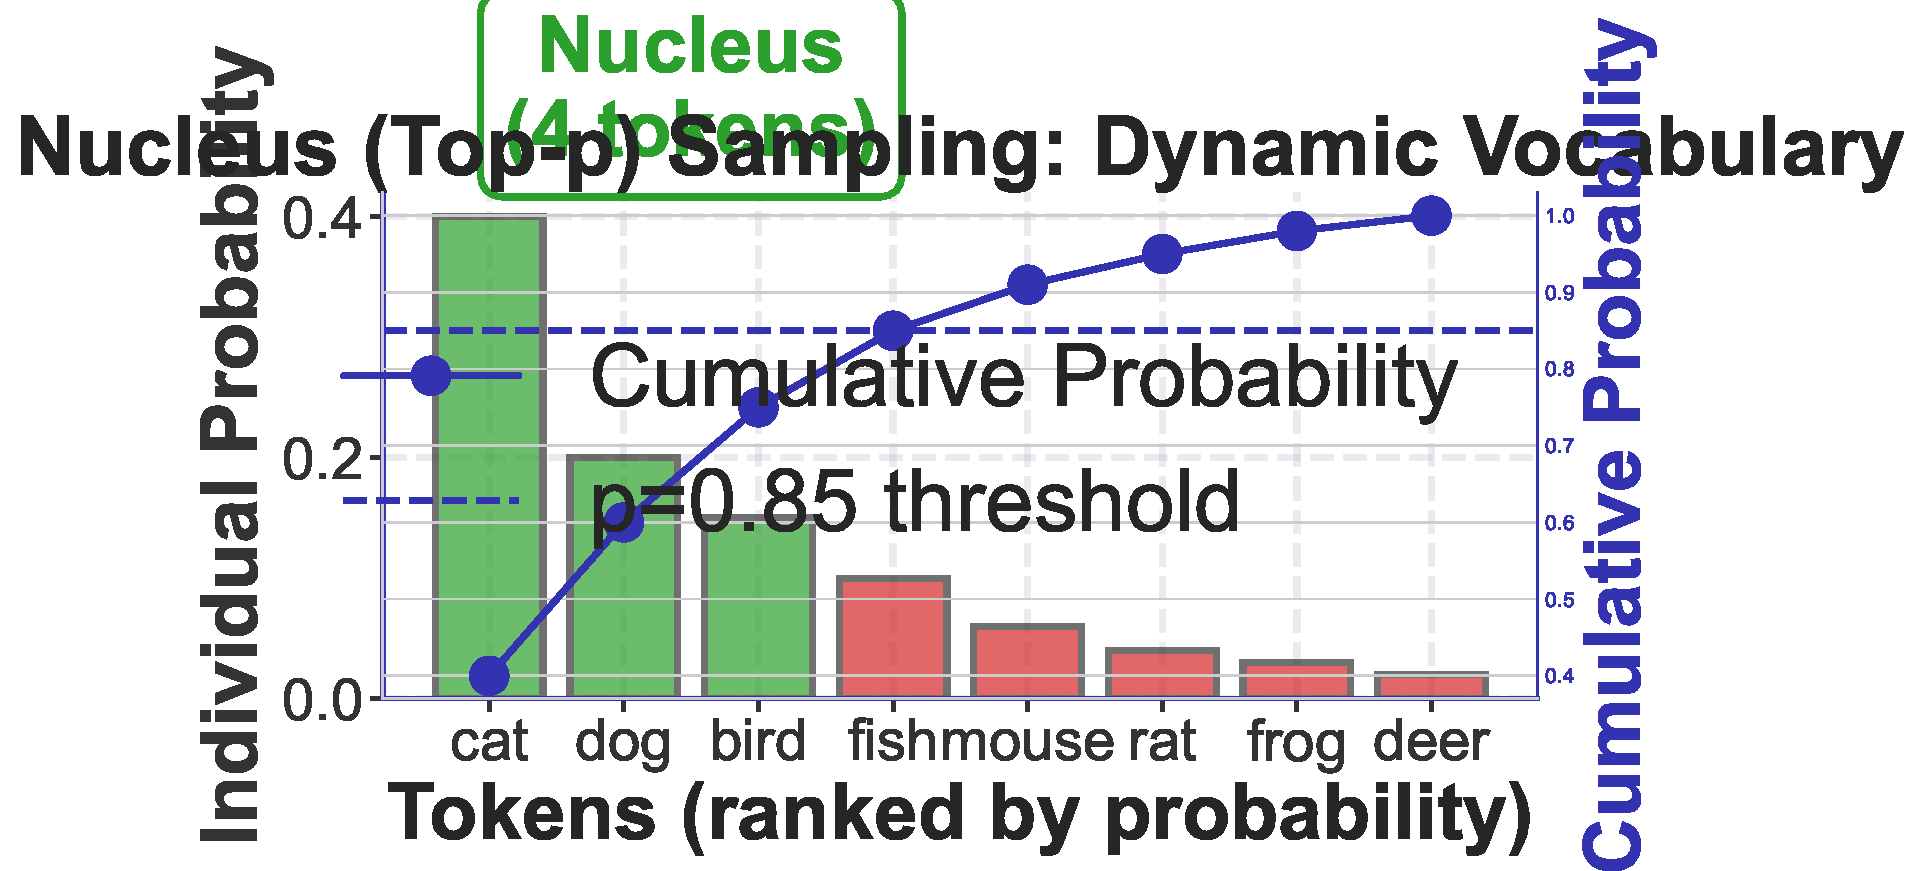
\includegraphics[width=0.70\textwidth]{../figures/nucleus_process_bsc.pdf}
\end{center}
\begin{center}
\textbf{Key Insight}: Adapt vocabulary size to distribution shape
\end{center}
\bottomnote{Nucleus size grows/shrinks based on probability spread}
\end{frame}

\begin{frame}[t]{Nucleus: How Distribution Shape Matters}
\vspace{-0.3cm}
\begin{center}
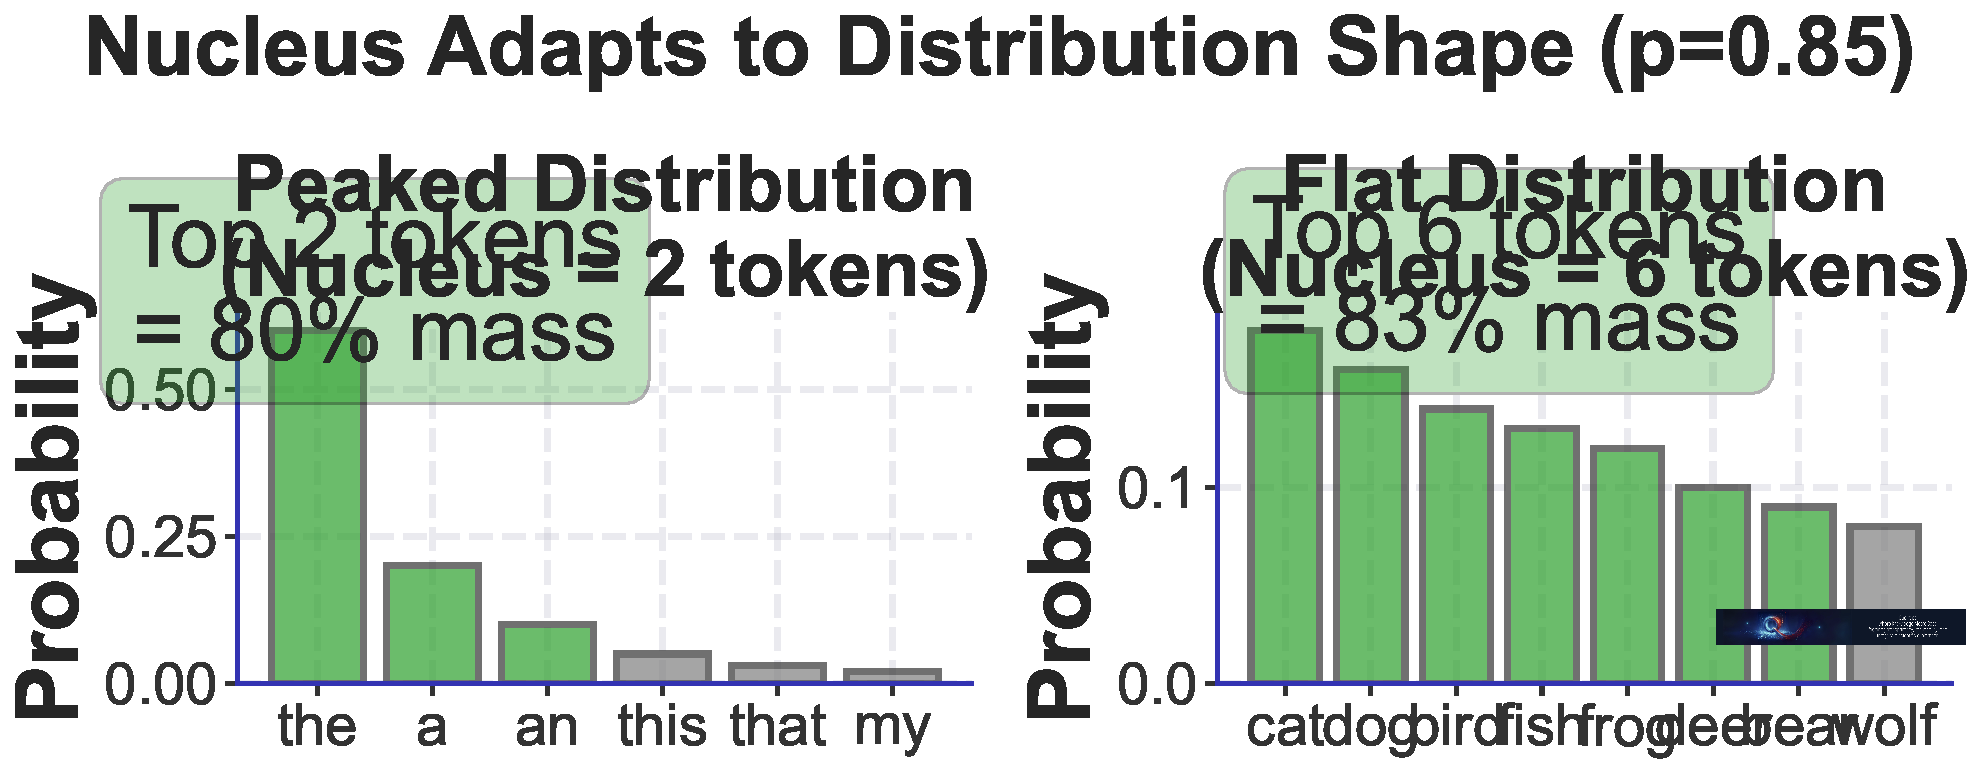
\includegraphics[width=0.70\textwidth]{../figures/nucleus_cumulative_bsc.pdf}
\end{center}
\bottomnote{Same p value gives different vocabulary sizes for peaked vs flat distributions}
\end{frame}

\begin{frame}[t]{Nucleus (Top-p): Detail}
\small
\begin{columns}[T]
\column{0.49\textwidth}
\textbf{Algorithm}:

\begin{enumerate}
\item Sort tokens by $P(w_i)$ (descending)
\item Compute cumulative sum: $\text{cum}_j = \sum_{i=1}^j p_i$
\item Find smallest set where $\text{cum} \geq p$
\item Sample from this nucleus
\end{enumerate}

\vspace{3mm}
\textbf{Example} (p=0.85):

Probs: [0.40, 0.20, 0.15, 0.10, ...]

Cumsum: [0.40, 0.60, 0.75, 0.85, ...]

Nucleus: First 4 tokens (0.85 $\geq$ 0.85)

\column{0.49\textwidth}
\textbf{Recommended Settings}:

\begin{itemize}
\item \textbf{p = 0.85-0.90}: Dialogue
\item \textbf{p = 0.90-0.95}: Creative writing
\item \textbf{p = 0.95-0.99}: Very diverse
\end{itemize}

\vspace{3mm}
\textbf{Why Better}:

Peaked distribution → small nucleus (2-3 tokens)

Flat distribution → large nucleus (10+ tokens)

Adapts automatically!

\vspace{3mm}
\textbf{Current Standard}: ChatGPT, Claude, GPT-4 all use nucleus

\end{columns}
\bottomnote{Nucleus sampling is the modern standard for high-quality generation}
\end{frame}

% === NEW: CONTRASTIVE SEARCH (3 slides: 16-18) ===

\begin{frame}[t]{The Degeneration Problem}
\vspace{-0.3cm}
\begin{center}
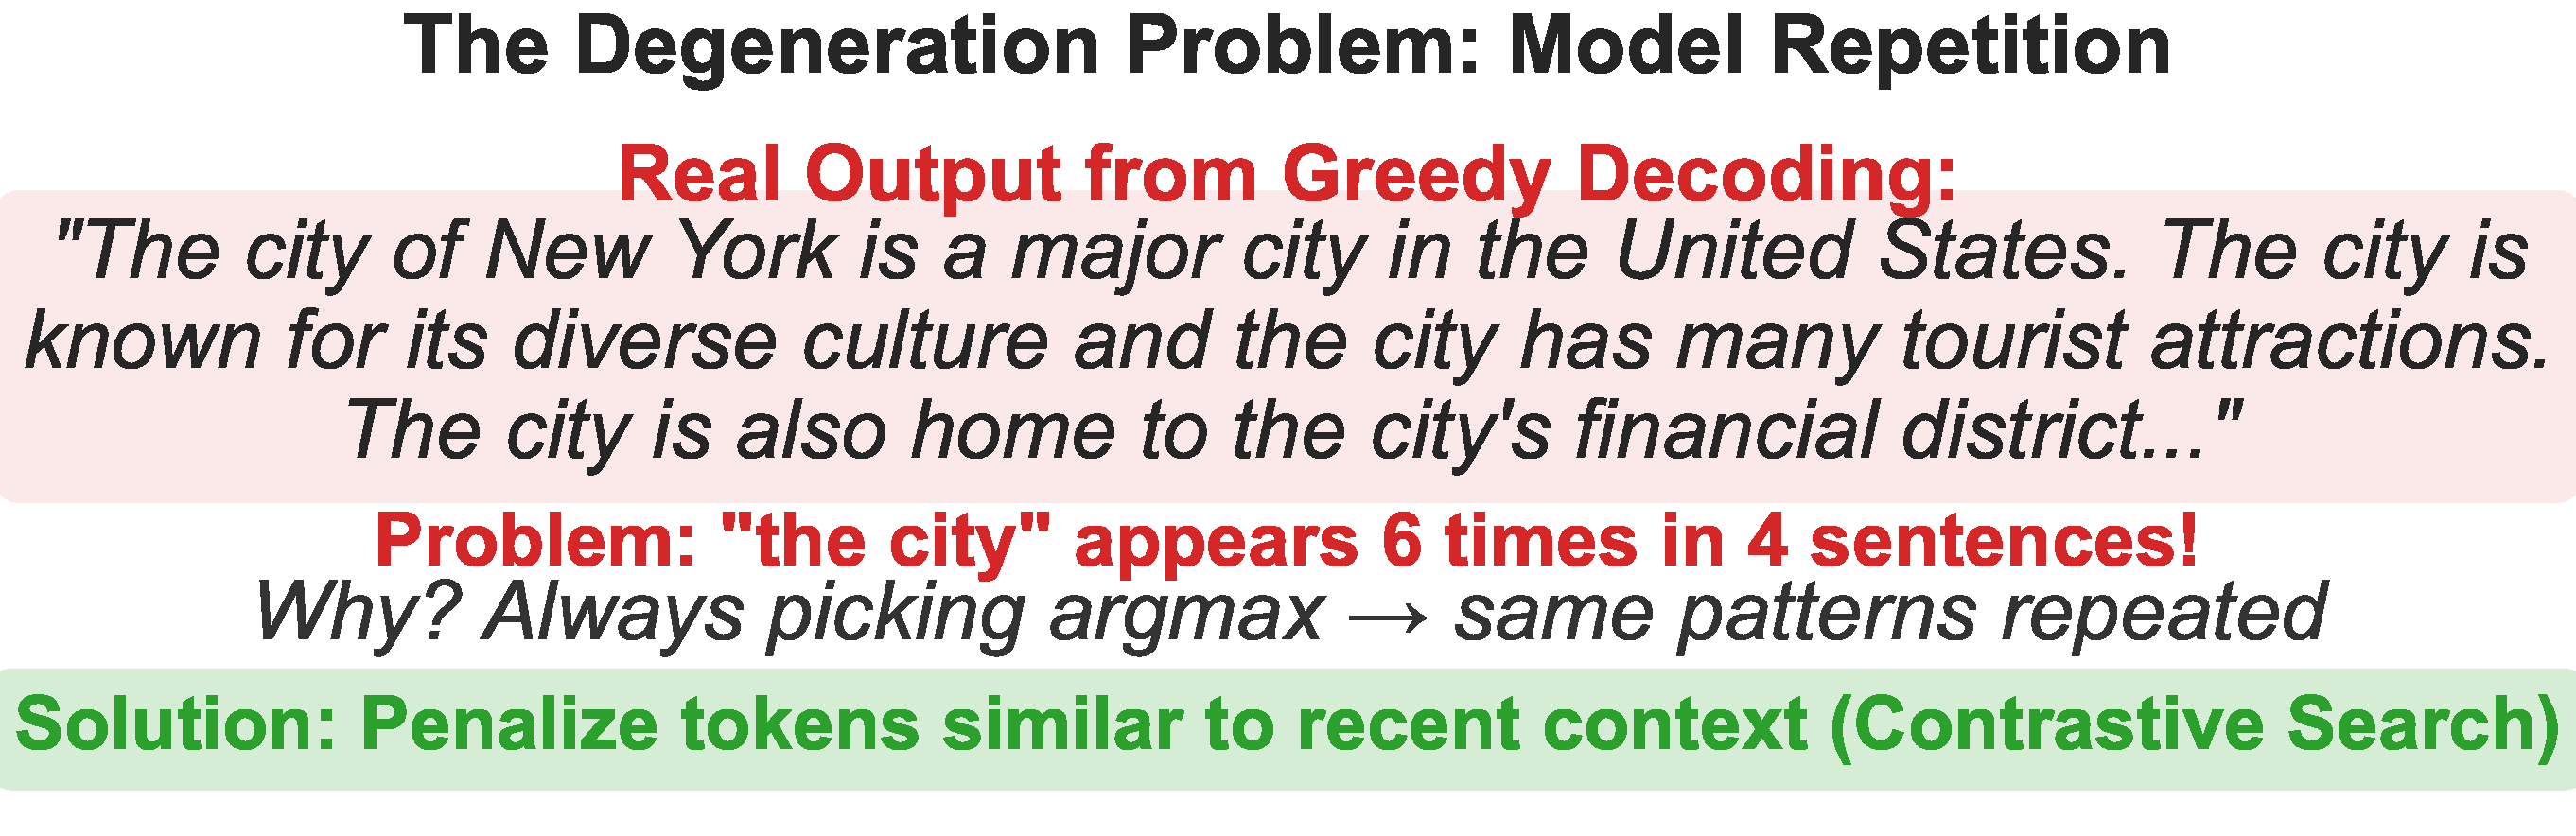
\includegraphics[width=0.70\textwidth]{../figures/degeneration_problem_bsc.pdf}
\end{center}
\begin{center}
\textbf{Discovery Question}: Why do models repeat themselves?
\end{center}
\bottomnote{Greedy and beam search maximize probability - but high probability = repeating recent context}
\end{frame}

\begin{frame}[t]{Contrastive Search: Penalize Repetition}
\vspace{-0.3cm}
\begin{center}
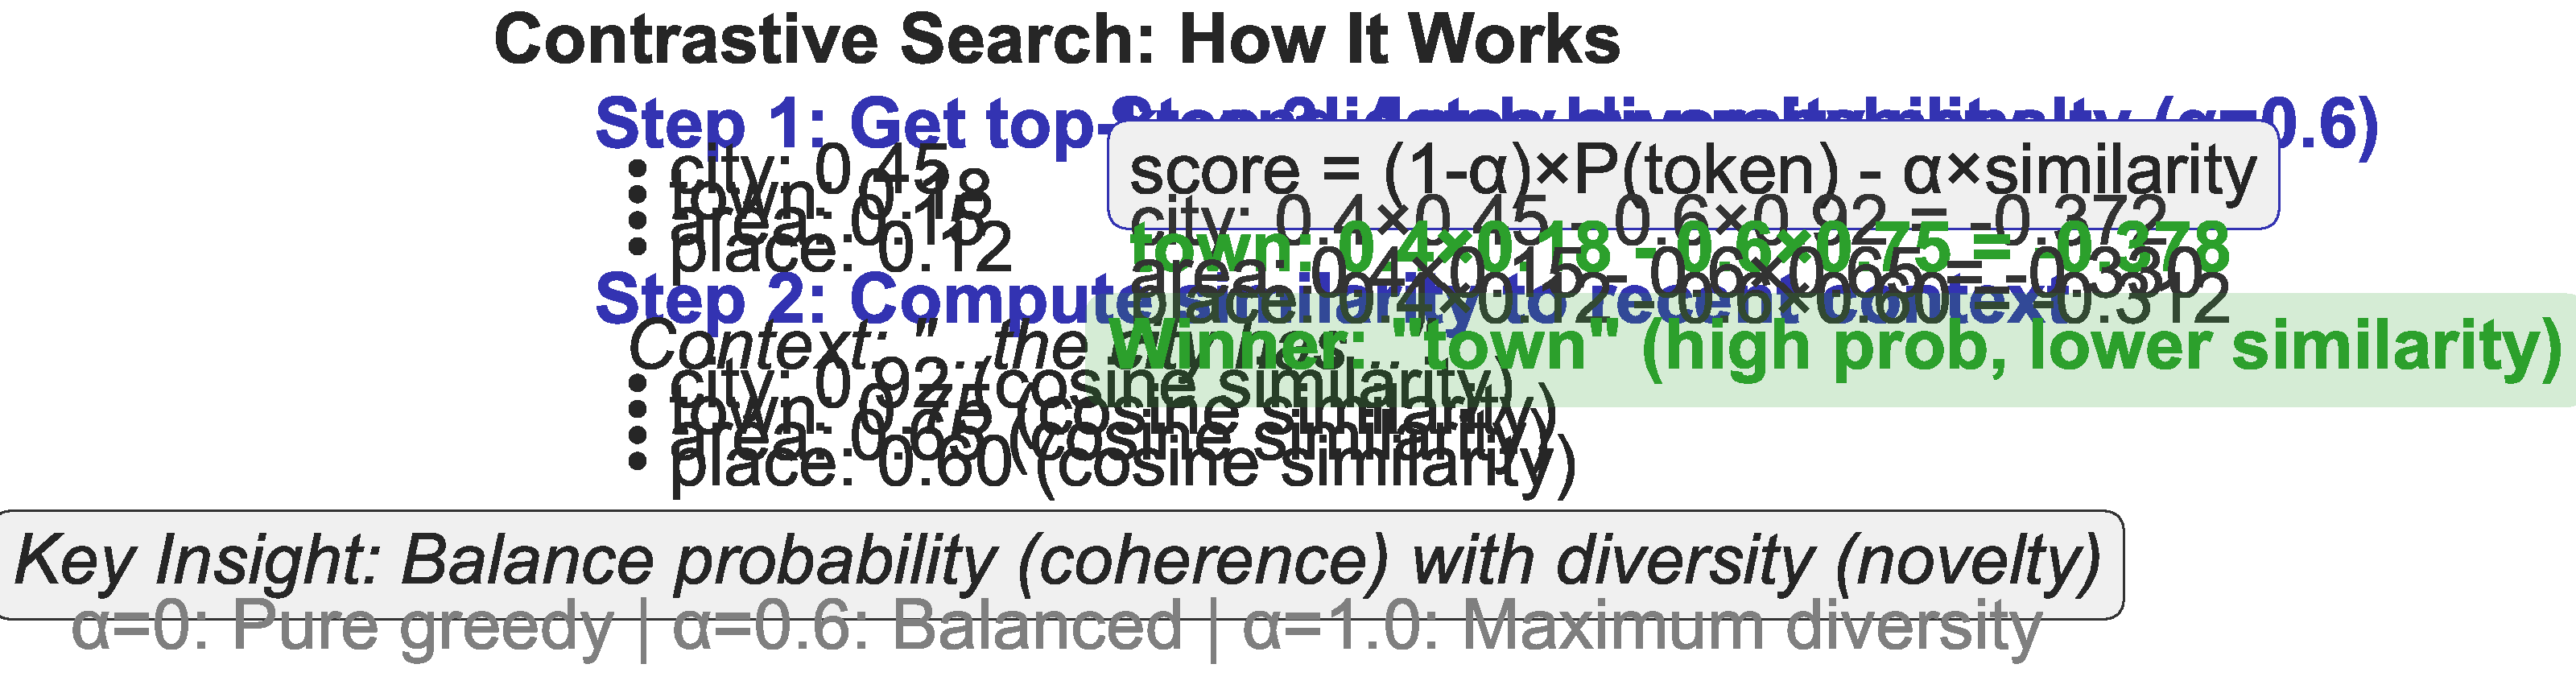
\includegraphics[width=0.70\textwidth]{../figures/contrastive_mechanism_bsc.pdf}
\end{center}
\begin{center}
\textbf{Key Insight}: Balance probability with diversity penalty
\end{center}
\bottomnote{Explicitly avoid copying recent context - prevents degeneration in long texts}
\end{frame}

\begin{frame}[t]{Contrastive vs Nucleus: Comparison}
\vspace{-0.3cm}
\begin{center}
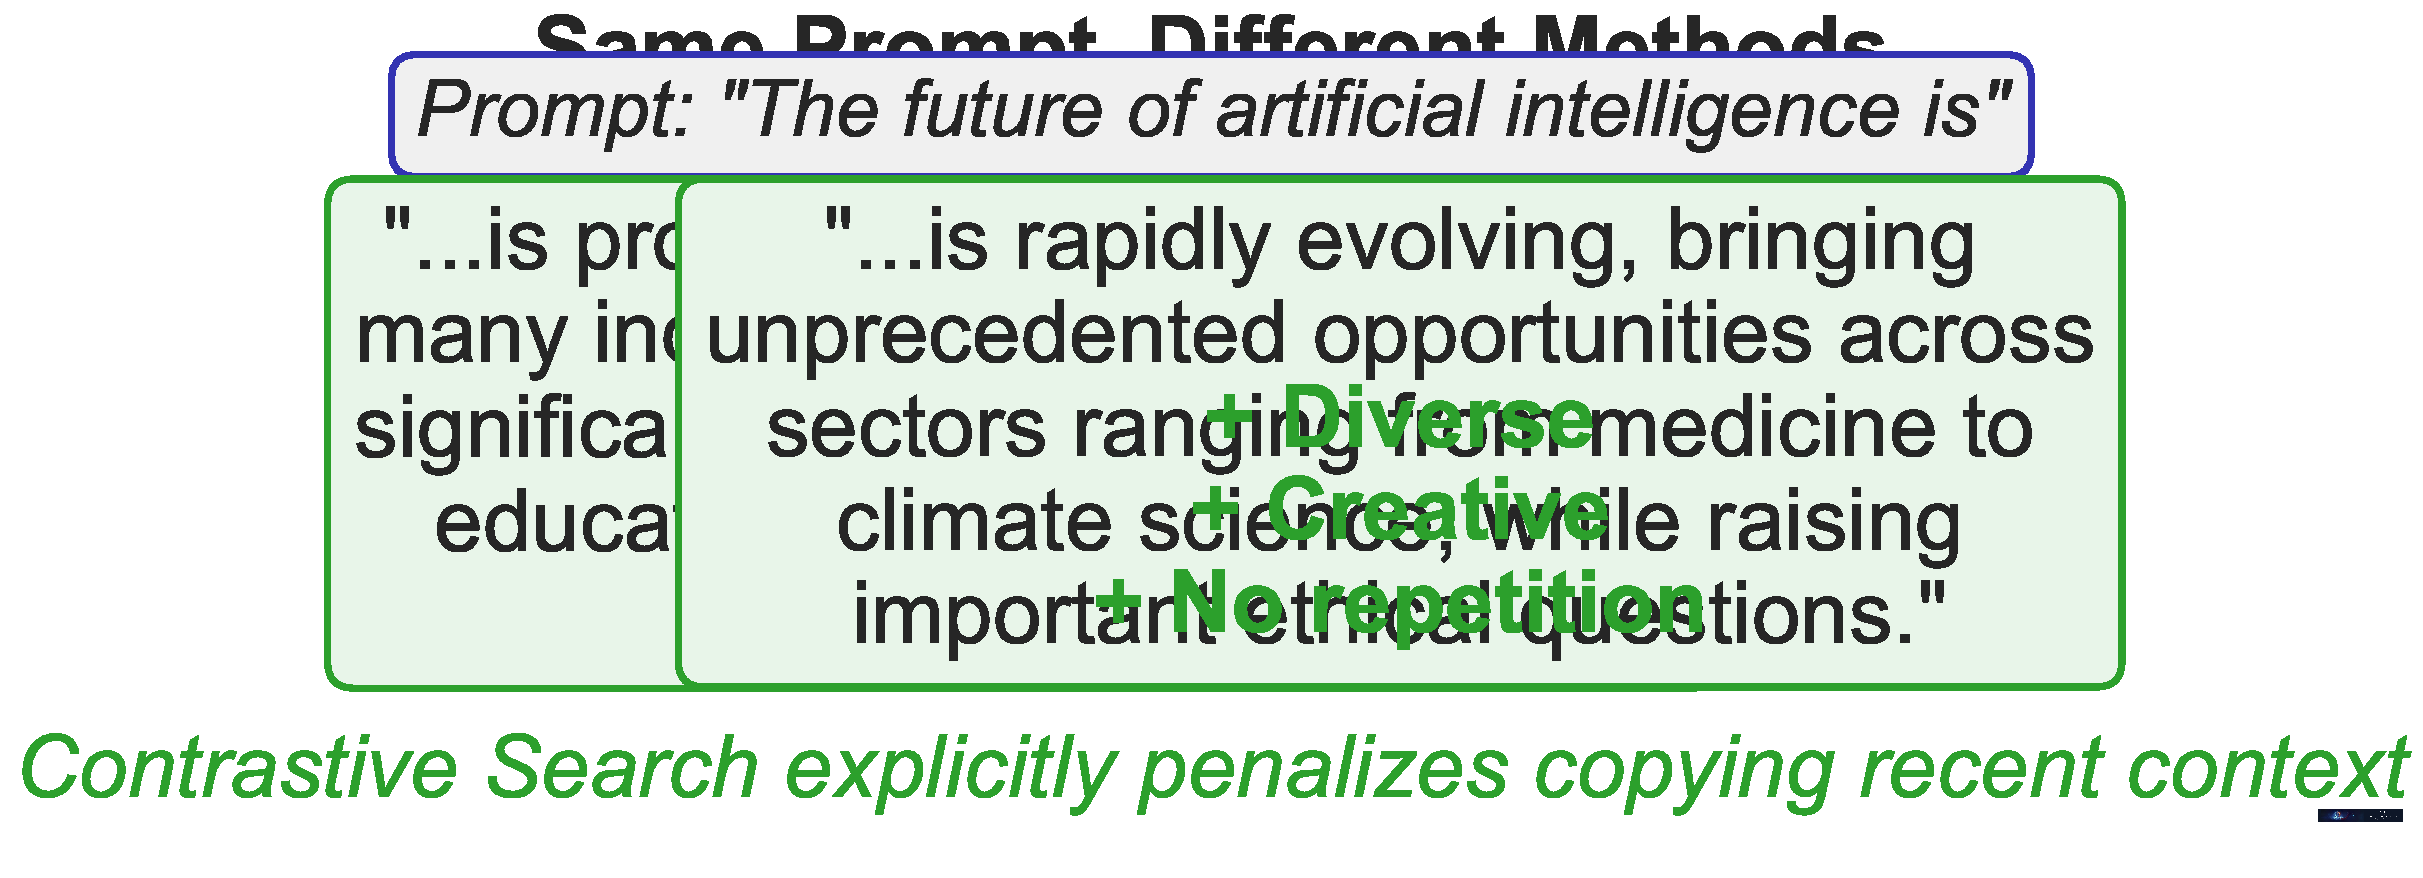
\includegraphics[width=0.75\textwidth]{../figures/contrastive_vs_nucleus_bsc.pdf}
\end{center}
\bottomnote{Contrastive search prevents repetition better than nucleus for long generation}
\end{frame}

% === QUALITY-DIVERSITY OPTIMIZATION (1 slide: 19) ===

\begin{frame}[t]{All Methods on Quality-Diversity Space}
\vspace{-0.3cm}
\begin{center}
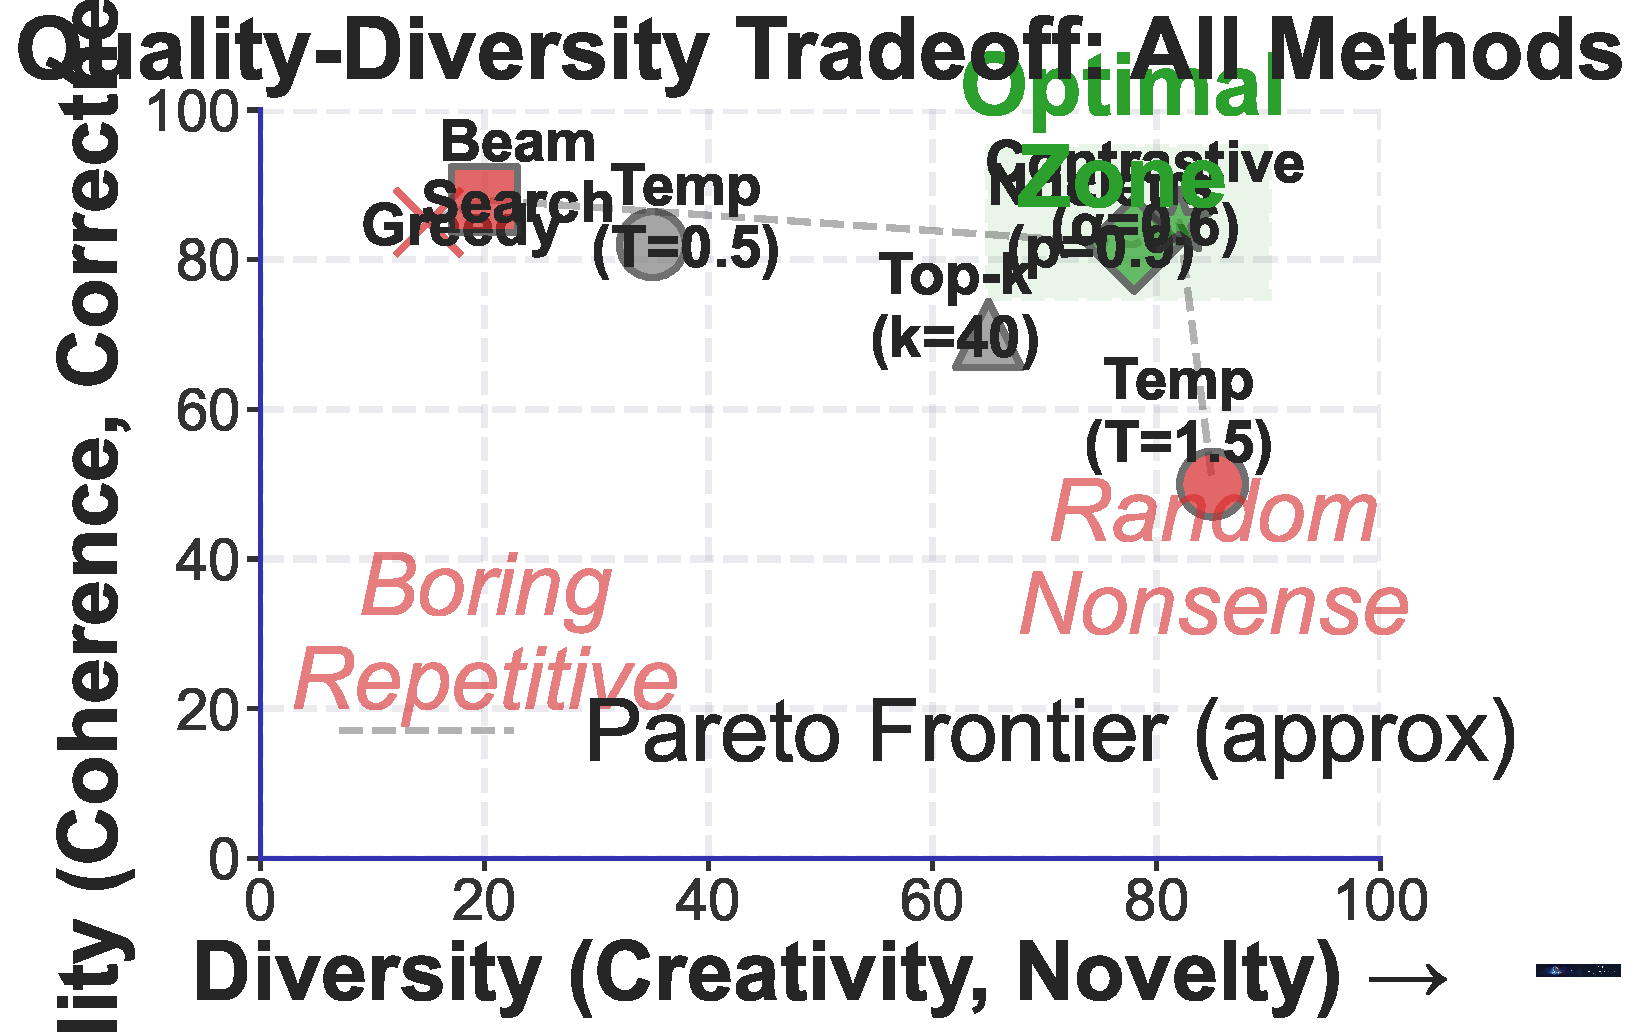
\includegraphics[width=0.70\textwidth]{../figures/quality_diversity_pareto_bsc.pdf}
\end{center}
\begin{center}
\textbf{Pareto Frontier}: No method dominates all others
\end{center}
\bottomnote{Choose based on task: deterministic tasks (left), creative tasks (right)}
\end{frame}

% === TASK-SPECIFIC RECOMMENDATIONS (3 slides: 20-22) ===

\begin{frame}[t]{Choosing the Right Method: Decision Tree}
\vspace{-0.3cm}
\begin{center}
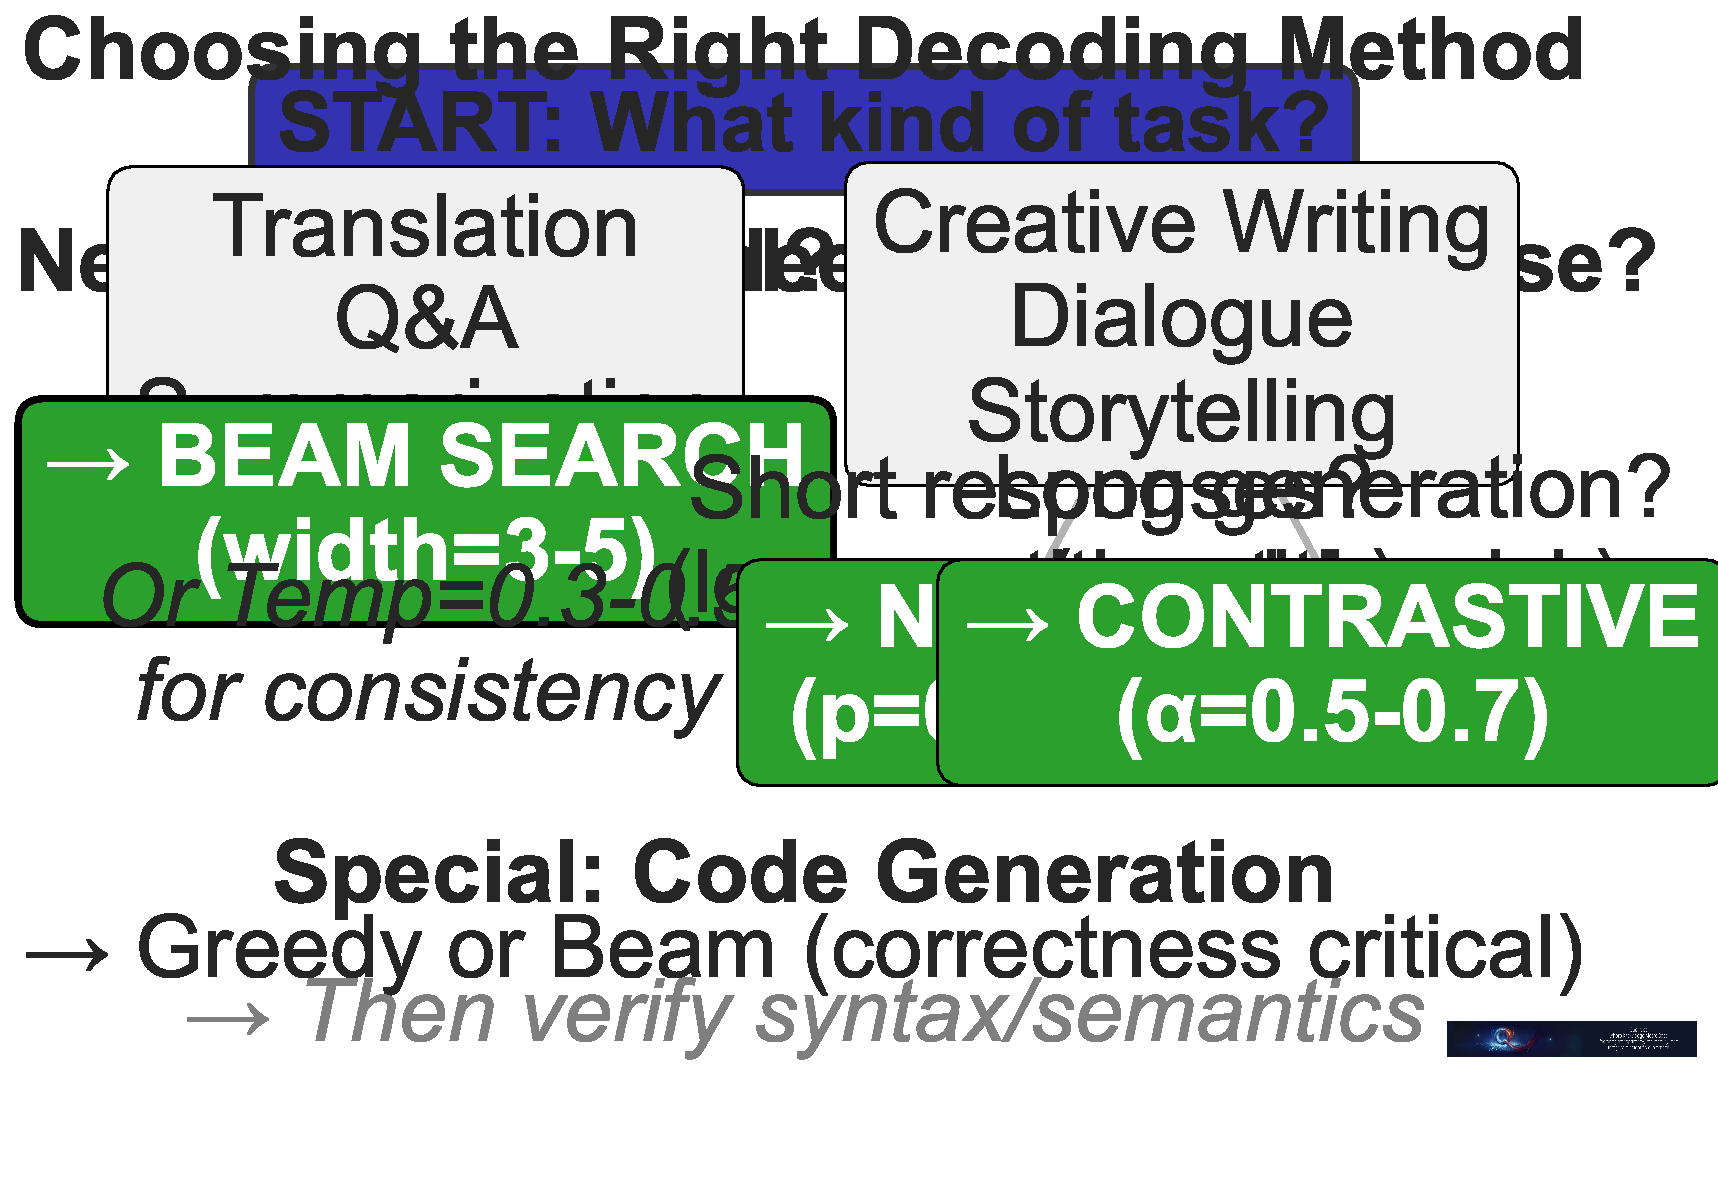
\includegraphics[width=0.70\textwidth]{../figures/task_method_decision_tree_bsc.pdf}
\end{center}
\bottomnote{Start with task requirements, follow tree to recommended method}
\end{frame}

\begin{frame}[t]{Task-Specific Recommendations (2025)}
\vspace{-0.3cm}
\begin{center}
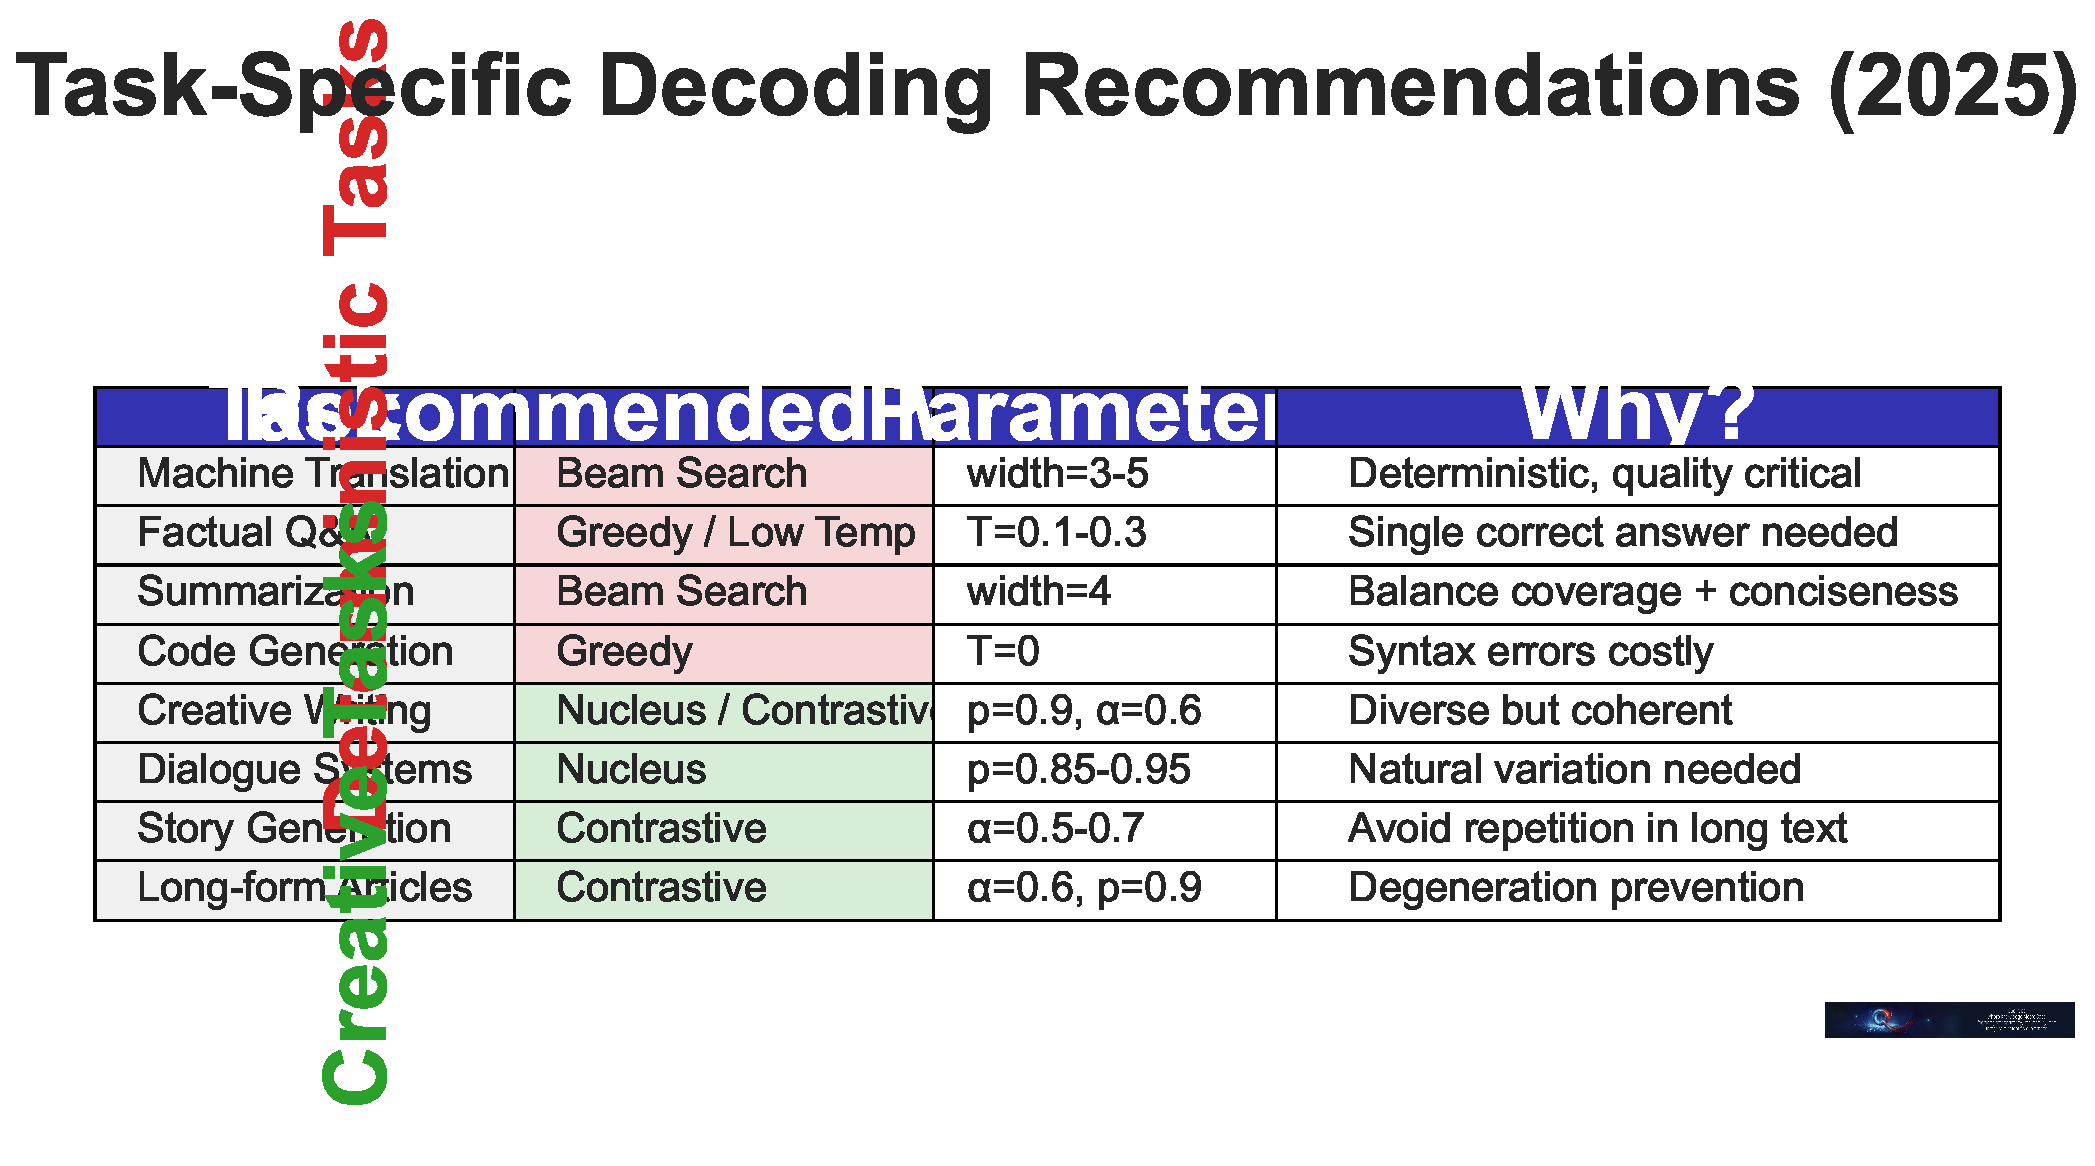
\includegraphics[width=0.75\textwidth]{../figures/task_recommendations_table_bsc.pdf}
\end{center}
\bottomnote{Comprehensive mapping from 8 common tasks to optimal decoding strategies}
\end{frame}

\begin{frame}[t]{Computational Costs Matter}
\vspace{-0.3cm}
\begin{center}
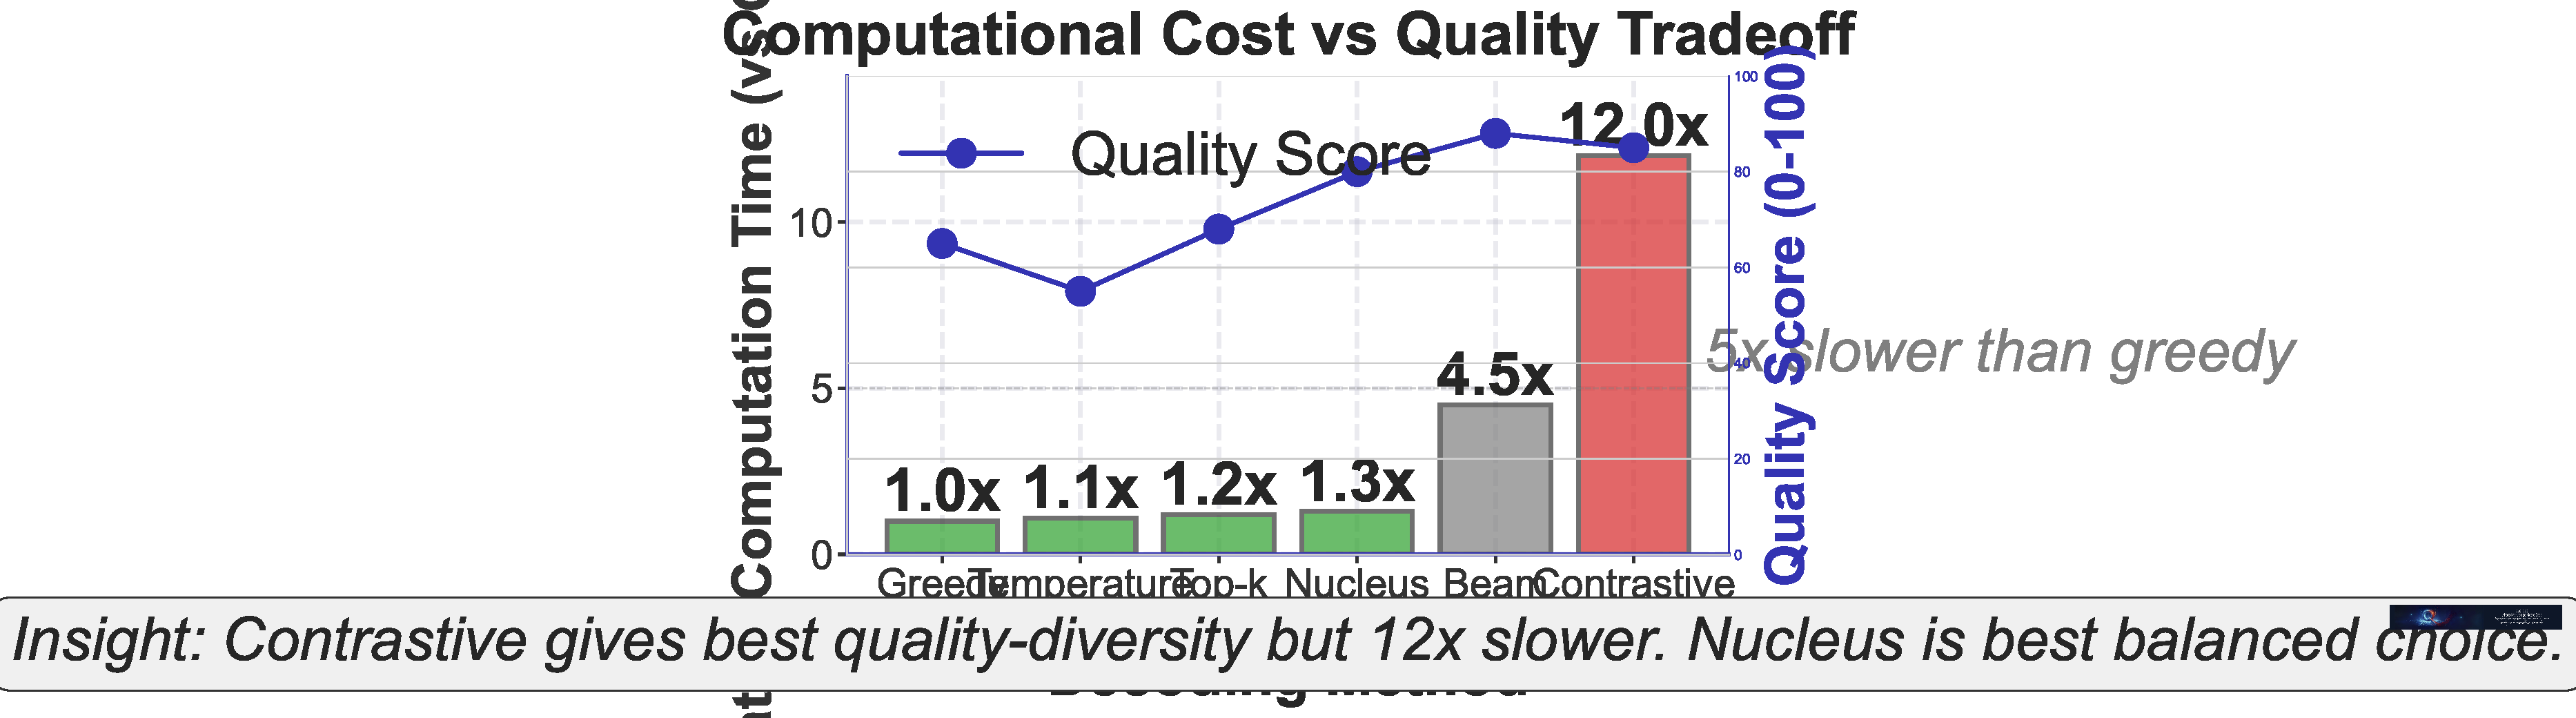
\includegraphics[width=0.70\textwidth]{../figures/computational_cost_comparison_bsc.pdf}
\end{center}
\begin{center}
\textbf{Tradeoff}: Contrastive gives best quality-diversity but 12× slower
\end{center}
\bottomnote{Nucleus is the best balanced choice for most applications}
\end{frame}

% === SUMMARY (1 slide: 23) ===

\begin{frame}[t]{Key Takeaways}
\begin{enumerate}
\item \textbf{Deterministic} (Greedy, Beam): High quality, no diversity - for factual tasks
\item \textbf{Temperature}: Simple randomness control - universal but crude
\item \textbf{Top-k}: Fixed vocabulary filter - prevents tail sampling
\item \textbf{Nucleus (Top-p)}: Dynamic cutoff - modern standard, adapts to distribution
\item \textbf{Contrastive}: Explicit degeneration prevention - best for long creative text
\item \textbf{Task matters}: Translation → Beam | Dialogue → Nucleus | Stories → Contrastive
\end{enumerate}

\vspace{5mm}
\textbf{Next}: Lab - Implement all 6 methods, measure quality-diversity tradeoffs

\bottomnote{Decoding strategy matters as much as model architecture}
\end{frame}

% ============================================
% TECHNICAL APPENDIX (19 SLIDES: A1-A19)
% ============================================

\begin{frame}[t]{}
\begin{center}
\Huge\textbf{Technical Appendix}

\vspace{1cm}
\large 19 slides: Complete mathematical treatment

\vspace{0.5cm}
\secondary{A1-A5: Beam Search Mathematics}

\secondary{A6-A10: Sampling Mathematics}

\secondary{A11-A14: Contrastive Search \& Degeneration}

\secondary{A15-A19: Advanced Topics \& Production}
\end{center}
\end{frame}

% === A1-A5: BEAM SEARCH MATHEMATICS ===

\begin{frame}[t]{A1: Beam Search Formulation}
\small
\textbf{Objective}: Find sequence $y^* = \argmax P(y | x)$

\vspace{3mm}
\textbf{Decomposition}:

$$P(y | x) = \prod_{t=1}^T P(y_t | y_{<t}, x)$$

\vspace{3mm}
\textbf{Log-probability} (more stable):

$$\log P(y | x) = \sum_{t=1}^T \log P(y_t | y_{<t}, x)$$

\vspace{3mm}
\textbf{Beam Search Approximation}:

Instead of exploring all $V^T$ sequences, maintain top-k hypotheses at each step

\vspace{3mm}
\textbf{Complexity}:

Time: $O(k \cdot V \cdot T)$ where $k$ = beam width, $V$ = vocabulary, $T$ = length

Space: $O(k \cdot T)$ to store hypotheses

\bottomnote{Beam search is tractable approximation to exact search}
\end{frame}

\begin{frame}[t]{A2: Length Normalization}
\small
\textbf{Problem}: Longer sequences have lower probabilities (more terms multiplied)

$$P(y_1, y_2, y_3, y_4) = \underbrace{0.5}_{y_1} \times \underbrace{0.5}_{y_2} \times \underbrace{0.5}_{y_3} \times \underbrace{0.5}_{y_4} = 0.0625$$

$$P(y_1, y_2) = 0.5 \times 0.5 = 0.25 > 0.0625$$

Bias toward shorter sequences!

\vspace{3mm}
\textbf{Solution}: Length normalization

$$\text{score}(y) = \frac{1}{|y|^\alpha} \log P(y)$$

where $\alpha \in [0.5, 1.0]$ (typically 0.6-0.7)

\vspace{3mm}
\textbf{Effect}:

Without: Beam search heavily biases toward short outputs

With: Fair comparison across different lengths

\bottomnote{Length normalization is essential for beam search quality}
\end{frame}

\begin{frame}[t]{A3: Beam Search Variants}
\small
\begin{columns}[T]
\column{0.49\textwidth}
\textbf{Diverse Beam Search}:

Partition beams into groups

Penalize within-group similarity

Result: More diverse hypotheses

\vspace{3mm}
\textbf{Constrained Beam Search}:

Force certain tokens to appear

Useful for: Keywords, entities

Applications: Controllable generation

\column{0.49\textwidth}
\textbf{Stochastic Beam Search}:

Sample beams instead of argmax

Combines beam + sampling

More diverse than standard beam

\vspace{3mm}
\textbf{Block n-gram Beam}:

Penalize n-gram repetition

Prevents ``the city is a city'' loops

Common in summarization

\end{columns}
\bottomnote{Many beam search variants exist for specific requirements}
\end{frame}

\begin{frame}[t]{A4: Beam Search Stopping Criteria}
\small
\textbf{When to stop expanding beams}?

\vspace{5mm}
\textbf{Method 1}: Fixed length

Stop at $T_{\max}$ tokens (simple but rigid)

\vspace{5mm}
\textbf{Method 2}: END token

Stop when beam generates special token (most common)

\vspace{5mm}
\textbf{Method 3}: Score threshold

Stop when best score cannot improve enough

$$\frac{\text{best\_incomplete}}{\text{best\_complete}} < \text{threshold}$$

\vspace{5mm}
\textbf{Method 4}: Timeout

Computational budget exceeded (production systems)

\bottomnote{Choice of stopping criterion affects output length distribution}
\end{frame}

\begin{frame}[t]{A5: Beam Search Limitations}
\small
\textbf{Fundamental Issues}:

\begin{enumerate}
\item \textbf{Exposure bias}: Trained with teacher forcing, tested with own outputs
\item \textbf{Label bias}: Cannot compare sequences of different prefixes fairly
\item \textbf{Repetition}: Still can loop (``the city is a major city'')
\item \textbf{Bland outputs}: Maximizes probability, not interestingness
\item \textbf{Search errors}: May miss better sequences outside beam
\end{enumerate}

\vspace{5mm}
\textbf{When Beam Search Fails}:

Open-ended generation (dialogue, stories)

Long-form text (repetition accumulates)

Creative tasks (probability $\neq$ quality)

\vspace{5mm}
→ Need sampling-based methods

\bottomnote{Beam search optimizes wrong objective for creative tasks}
\end{frame}

% === A6-A10: SAMPLING MATHEMATICS ===

\begin{frame}[t]{A6: Sampling as Inference}
\small
\textbf{Goal}: Sample $y \sim P(y | x)$ instead of $\argmax P(y | x)$

\vspace{3mm}
\textbf{Ancestral Sampling}:

For $t = 1$ to $T$:

\hspace{1cm} Compute $P(y_t | y_{<t}, x)$

\hspace{1cm} Sample $y_t \sim P(\cdot | y_{<t}, x)$

\vspace{3mm}
\textbf{Properties}:

Stochastic: Different output each time

Explores full distribution (in expectation)

Can generate low-probability sequences

\vspace{3mm}
\textbf{Variants}:

Temperature: Reshape distribution before sampling

Top-k: Truncate distribution before sampling

Nucleus: Dynamic truncation before sampling

\bottomnote{Sampling enables diversity but loses quality guarantees}
\end{frame}

\begin{frame}[t]{A7: Temperature Mathematics}
\small
\textbf{Softmax with Temperature}:

$$p_i(T) = \frac{\exp(z_i / T)}{\sum_{j=1}^V \exp(z_j / T)}$$

\vspace{3mm}
\textbf{Limiting Cases}:

$T \rightarrow 0$: $p_i \rightarrow \begin{cases} 1 & \text{if } i = \argmax z \\ 0 & \text{otherwise} \end{cases}$ (greedy)

$T \rightarrow \infty$: $p_i \rightarrow 1/V$ (uniform)

\vspace{3mm}
\textbf{Entropy Analysis}:

Entropy $H(p) = -\sum p_i \log p_i$ measures randomness

$H$ increases monotonically with $T$

Low $T$ ($<$0.5): $H \approx 0$ (deterministic)

High $T$ ($>$2.0): $H \approx \log V$ (maximum entropy)

\bottomnote{Temperature provides continuous control over distribution entropy}
\end{frame}

\begin{frame}[t]{A8: Top-k Mathematics}
\small
\textbf{Formal Definition}:

Let $\sigma$ = permutation sorting probabilities descending

$$V_k = \{w_{\sigma(1)}, w_{\sigma(2)}, ..., w_{\sigma(k)}\}$$

Truncated distribution:

$$p'(w) = \begin{cases} \frac{p(w)}{\sum_{w' \in V_k} p(w')} & \text{if } w \in V_k \\ 0 & \text{otherwise} \end{cases}$$

\vspace{3mm}
\textbf{Information Loss}:

Original entropy: $H(p) = -\sum_{i=1}^V p_i \log p_i$

After top-k: $H(p') = -\sum_{i=1}^k p'_i \log p'_i < H(p)$

Loss $\approx \sum_{i=k+1}^V p_i \log(1/p_i)$ (tail information)

\bottomnote{Top-k sacrifices tail probability mass for sampling quality}
\end{frame}

\begin{frame}[t]{A9: Nucleus (Top-p) Mathematics}
\small
\textbf{Formal Definition}:

$$V_p = \min \left\{ V' \subseteq V : \sum_{w \in V'} p(w) \geq p \right\}$$

Smallest set with cumulative mass $\geq p$

\vspace{3mm}
\textbf{Dynamic Vocabulary Size}:

$$|V_p| = \min \{k : \sum_{i=1}^k p_{\sigma(i)} \geq p\}$$

Adapts to distribution shape:

Peaked: Small $|V_p|$ (2-5 tokens)

Flat: Large $|V_p|$ (50+ tokens)

\vspace{3mm}
\textbf{Why Nucleus $>$ Top-k}:

Top-k: Fixed $k$ regardless of $p(w)$ distribution

Nucleus: Adapts $k$ to achieve consistent probability mass

\bottomnote{Nucleus automatically adjusts vocabulary to distribution characteristics}
\end{frame}

\begin{frame}[t]{A10: Sampling Quality Metrics}
\small
\begin{columns}[T]
\column{0.49\textwidth}
\textbf{Quality Metrics}:

\textbf{Perplexity}: $\exp(-\frac{1}{T} \sum \log p(y_t))$

Lower = better

\vspace{3mm}
\textbf{BLEU} (translation):

N-gram overlap with reference

0-100 scale

\vspace{3mm}
\textbf{Human evaluation}:

Fluency (1-5)

Relevance (1-5)

\column{0.49\textwidth}
\textbf{Diversity Metrics}:

\textbf{Distinct-n}: $\frac{\text{unique n-grams}}{\text{total n-grams}}$

Higher = more diverse

\vspace{3mm}
\textbf{Self-BLEU}:

BLEU of output vs other outputs

Lower = more diverse

\vspace{3mm}
\textbf{Repetition Rate}:

$\frac{\text{repeated n-grams}}{\text{total n-grams}}$

Lower = less repetitive

\end{columns}
\bottomnote{Need both quality AND diversity metrics to evaluate decoding}
\end{frame}

% === A11-A14: CONTRASTIVE SEARCH & DEGENERATION ===

\begin{frame}[t]{A11: The Degeneration Problem (Formal)}
\small
\textbf{Definition}: Model-generated text with unnatural repetitions

\vspace{3mm}
\textbf{Why It Happens}:

\begin{enumerate}
\item Model trained on natural text (low repetition)
\item But generation maximizes $P(y_t | y_{<t})$
\item Recent context $y_{<t}$ influences $P$
\item Creates positive feedback: high prob word → context → same high prob word
\end{enumerate}

\vspace{3mm}
\textbf{Quantifying Degeneration}:

Repetition rate in greedy: 15-30\% (depending on domain)

Repetition rate in human text: 2-5\%

Gap = degeneration problem

\vspace{3mm}
\textbf{Examples}:

``\textit{The city is a major city in the United States. The city...}''

``\textit{I think that I think that I think...}''

\bottomnote{Maximizing probability does not equal natural text}
\end{frame}

\begin{frame}[t]{A12: Contrastive Search Objective}
\small
\textbf{Scoring Function}:

$$\text{score}(w_t) = (1 - \alpha) \times \underbrace{P(w_t | y_{<t})}_{\text{model confidence}} - \alpha \times \underbrace{\max_{w_i \in y_{<t}} \text{sim}(w_t, w_i)}_{\text{context similarity}}$$

where $\alpha \in [0, 1]$ controls tradeoff

\vspace{3mm}
\textbf{Similarity Function}:

$$\text{sim}(w_i, w_j) = \frac{h_i \cdot h_j}{||h_i|| \cdot ||h_j||}$$ (cosine similarity)

using token embeddings $h$

\vspace{3mm}
\textbf{Algorithm}:

\begin{enumerate}
\item Get top-k candidates by probability
\item For each candidate, compute similarity to all tokens in $y_{<t}$
\item Apply penalty: score = prob - $\alpha \times$ max\_similarity
\item Select candidate with highest score
\end{enumerate}

\bottomnote{Contrastive search explicitly penalizes copying recent context}
\end{frame}

\begin{frame}[t]{A13: Contrastive Search Parameters}
\small
\begin{columns}[T]
\column{0.49\textwidth}
\textbf{Alpha} ($\alpha$):

$\alpha = 0$: Pure greedy (no penalty)

$\alpha = 0.6$: Balanced (recommended)

$\alpha = 1.0$: Maximum diversity (risky)

\vspace{3mm}
\textbf{Typical Settings}:

Short text ($<$100 tokens): $\alpha = 0.4-0.5$

Medium ($<$500): $\alpha = 0.5-0.6$

Long (500+): $\alpha = 0.6-0.7$

\column{0.49\textwidth}
\textbf{Top-k for Candidates}:

$k = 4$: Fast, focused

$k = 6$: Balanced (default)

$k = 10$: Diverse

\vspace{3mm}
\textbf{Computational Cost}:

For each step:
\begin{itemize}
\item Compute similarities: $O(k \times t)$
\item $t$ grows with generation
\end{itemize}

Total: $O(k \times T^2)$

12× slower than greedy

\end{columns}
\bottomnote{Hugging Face default: $\alpha$=0.6, k=4}
\end{frame}

\begin{frame}[t]{A14: Degeneration Analysis}
\small
\textbf{Research Findings} (2024-2025):

\begin{itemize}
\item Greedy decoding repetition: 18-25\% (GPT-2), 12-18\% (GPT-3)
\item Nucleus sampling repetition: 8-12\% (still above human 3-5\%)
\item Contrastive search repetition: 4-7\% (closest to human)
\end{itemize}

\vspace{3mm}
\textbf{Why Probability Maximization Fails}:

Training objective: Next token prediction

But generation requires: Global coherence

Mismatch: Local optimum $\neq$ global quality

\vspace{3mm}
\textbf{Solutions Hierarchy}:

\begin{enumerate}
\item Temperature/Top-k/Nucleus: Reduce greedy's determinism
\item Contrastive: Explicit degeneration penalty
\item RLHF/DPO: Align model with human preferences (different lecture)
\end{enumerate}

\bottomnote{Contrastive search addresses fundamental limitation of likelihood-based decoding}
\end{frame}

% === A15-A19: ADVANCED TOPICS ===

\begin{frame}[t]{A15: Hybrid Decoding Methods}
\small
\textbf{Combining Strategies}:

\vspace{3mm}
\textbf{Nucleus + Temperature}:

Apply temperature THEN nucleus

$$p_i(T) = \softmax(z / T), \quad \text{then} \quad V_p \gets \text{nucleus}(p_i(T))$$

Used by GPT-3 API, ChatGPT

\vspace{3mm}
\textbf{Beam + Sampling}:

Beam search with stochastic selection

Keep top-k, sample from them (not argmax)

\vspace{3mm}
\textbf{Contrastive + Nucleus}:

Nucleus for candidate generation

Contrastive scoring for selection

Best of both worlds

\bottomnote{Hybrid methods leverage complementary strengths}
\end{frame}

\begin{frame}[t]{A16: Constrained Decoding (2025)}
\small
\textbf{Goal}: Force certain tokens/patterns to appear

\vspace{3mm}
\textbf{Lexically Constrained}:

Must include keywords: \{``AI'', ``ethics'', ``safety''\}

Beam search variant: Track constraint satisfaction

\vspace{3mm}
\textbf{Format Constraints}:

JSON output: Force structure \{``key'': ``value''\}

Code: Force syntactic validity

\vspace{3mm}
\textbf{NeuroLogic Decoding} (2021):

Beam search + constraint satisfaction

Optimal for: Keyword-based generation

\vspace{3mm}
\textbf{Production Use Cases}:

Structured data extraction (force JSON)

Controllable summarization (force keywords)

Code generation (force syntax)

\bottomnote{Constrained decoding enables controllable generation}
\end{frame}

\begin{frame}[t]{A17: Computational Complexity Comparison}
\small
\begin{center}
\begin{tabular}{lccc}
\hline
\textbf{Method} & \textbf{Time per token} & \textbf{Total complexity} & \textbf{Relative speed} \\
\hline
Greedy & $O(V)$ & $O(V \times T)$ & 1.0× (baseline) \\
Temperature & $O(V)$ & $O(V \times T)$ & 1.1× (softmax overhead) \\
Top-k & $O(V)$ & $O(V \times T)$ & 1.2× (sorting) \\
Nucleus & $O(V \log V)$ & $O(V \log V \times T)$ & 1.3× (sort + cumsum) \\
Beam (k=5) & $O(k \times V)$ & $O(k \times V \times T)$ & 4.5× (k=5) \\
Contrastive & $O(k \times T)$ & $O(k \times T^2)$ & 12× (similarity) \\
\hline
\end{tabular}
\end{center}

\vspace{3mm}
\textbf{Key Insight}: Contrastive's $T^2$ term makes it expensive for long sequences

\vspace{3mm}
\textbf{Practical Impact} (1000-token generation):

Greedy: 2.5 seconds

Nucleus: 3.2 seconds (best choice)

Beam: 11 seconds

Contrastive: 30 seconds (only if quality critical)

\bottomnote{Computational cost matters for production deployment}
\end{frame}

\begin{frame}[t]{A18: Production Deployment Settings (2024-2025)}
\vspace{-0.3cm}
\begin{center}
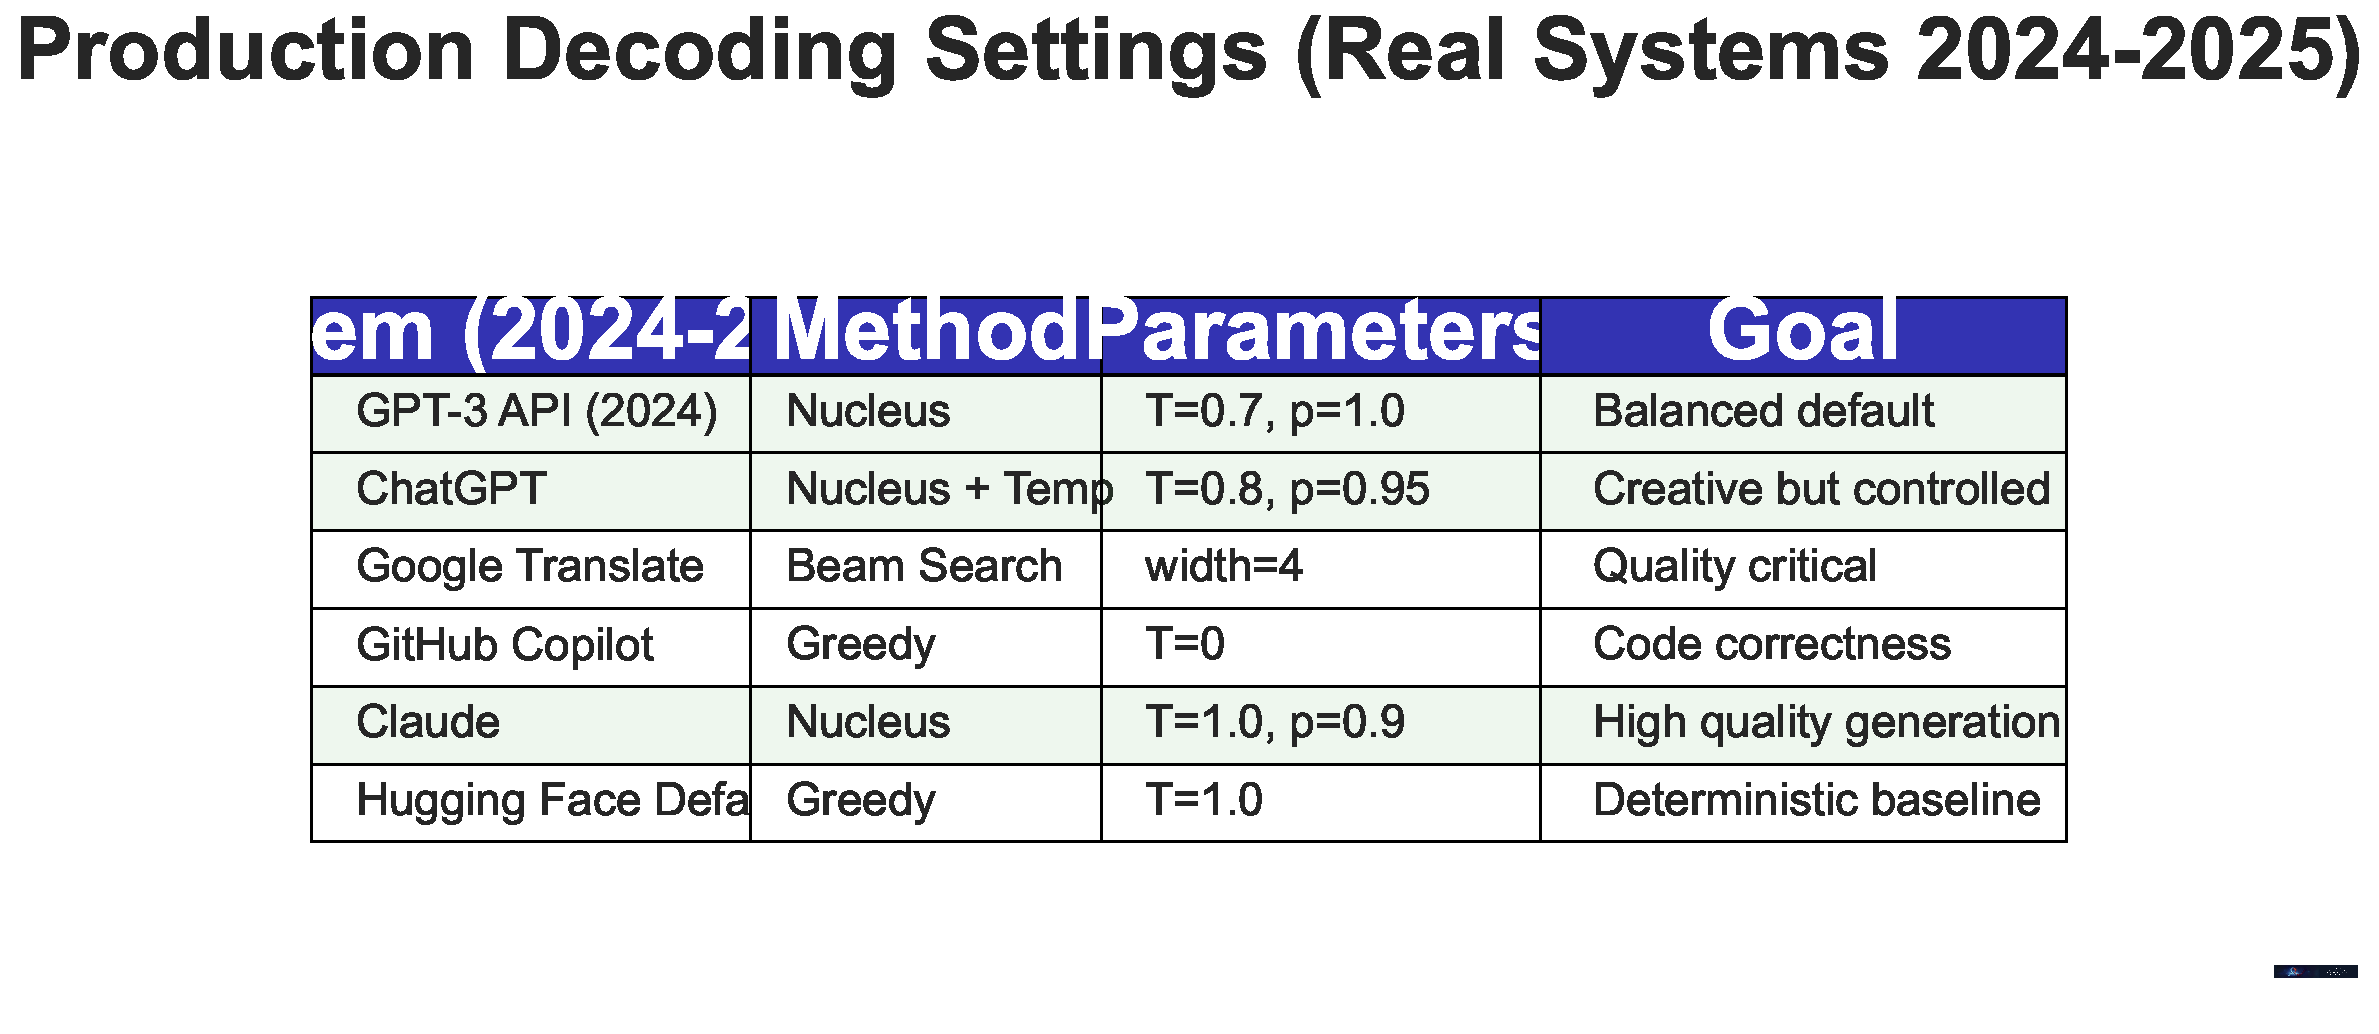
\includegraphics[width=0.75\textwidth]{../figures/production_settings_bsc.pdf}
\end{center}
\bottomnote{Real-world settings from major production systems}
\end{frame}

\begin{frame}[t]{A19: Future Directions \& Open Problems}
\small
\textbf{Active Research Areas} (2025):

\begin{enumerate}
\item \textbf{Quality-diversity optimization}: Multi-objective search methods
\item \textbf{Learned decoding}: Train models to decode better (RLHF, DPO)
\item \textbf{Speculative decoding}: Parallel generation for speed (4-8× faster)
\item \textbf{Adaptive methods}: Choose strategy dynamically during generation
\item \textbf{Energy-based decoding}: Score sequences globally (not token-by-token)
\end{enumerate}

\vspace{5mm}
\textbf{Open Problems}:

How to automatically select best $T$, $p$, $k$, $\alpha$ for new task?

How to balance fluency + factuality + creativity simultaneously?

How to decode efficiently for 100K+ token outputs?

\vspace{5mm}
\textbf{Trend}: Moving from hand-tuned parameters to learned decoding strategies

\bottomnote{Decoding is an active research area with many open questions}
\end{frame}

\end{document}
